\documentclass[pdftex,letterpaper,11pt]{article}%
\usepackage[export]{adjustbox}
\usepackage{multirow}
\usepackage[arabicsections]{dpugatex}
%\usepackage{dpppl}
%\usepackage{lscape}
\usepackage{pdflscape}
\usepackage{longtable}

\usepackage{tikz}

\usepackage[british]{babel}
\usepackage{amssymb,amsmath,warpcol,url,ctable,multirow,caption,threeparttable,float,soul,gensymb}
%\usepackage[noend]{algpseudocode}
\makeatletter
\def\BState{\State\hskip-\ALG@thistlm}
\makeatother


\usepackage{subcaption}


\usepackage{xcolor,colortbl}%Per colorejar cel·les de les taules
\definecolor{verylightgray}{gray}{0.90}
\newcommand{\verylightgray}[1]{\cellcolor{verylightgray}#1}


\usepackage{arydshln} %Per dashed lines
\setlength\dashlinedash{1.5pt}
\setlength\dashlinegap{2.5pt}
\setlength\arrayrulewidth{0.8pt}

\usepackage[utf8]{inputenc}
\usepackage{eurosym}
\usepackage{soul}
\setstcolor{red} % Tatxat vermell pel text a eliminar!!!!
\definecolor{lightgreen}{rgb}{0.564706,0.933333,0.564706}
\newcommand{\miquel}[1]{{\sethlcolor{lightgreen} \hl{#1}} } % To highlight with light green Miquel's comments.
\soulregister\citet7 % These \soulregister commands allow us to avoid problems between soul functions (\hl, \st, ...) and these other functions (\citet,\citep,\ref,\footnote, ...). Include more if it is necessary.
\soulregister\citep7
\soulregister\cite7
\soulregister\ref7
\soulregister\footnote7
\soulregister\textit7
\soulregister\textbf7
\soulregister\textsc7
\soulregister\`7 % for open accents.
\soulregister\'7 % for closed accents.
\soulregister\% 7 % for \%age symbol
\usepackage{tabularx,tabulary}
\usepackage[osf]{mathpazo} % Amb aquest paquet faig ús de la lletra Palatino, la que fan servir Puga, Duranton et al. Amb l'opció [osf] la numeració és "old fashion", però és incompatible amb un títol en negreta i small caps (desapareixen les small caps!). Per tant, per ara opto per NO aplicar aquesta opció.
\usepackage[abs]{overpic}

\usepackage{hyperref}
\definecolor{darkblue}{rgb}{0.0,0.0,0.3}
\hypersetup{colorlinks=true, breaklinks=true, citecolor= darkblue, linkcolor=blue, urlcolor=blue}

\usepackage{chngcntr}

\newcommand{\mc}[3]{\multicolumn{#1}{#2}{#3}}
\newcommand{\mcc}[1]{\multicolumn{1}{c}{#1}}
\newcommand{\mcb}[1]{\multicolumn{1}{c}{\bf #1}}

\newcommand{\mr}[3]{\multirow{#1}{#2}{#3}} % Per fer Files múltiples (seguint el punt de vista de les columnes múltiples.
\newcommand{\mg}[3]{\multicolumn{#1}{#2}{\verylightgray #3}} %Combino el color de les cel·les amb al command de les columnes múltiples.



%\hypersetup{%
 % pdftitle={Race and neighborhoods in the 21$^{\text{st}}$ century},%
 % pdfauthor={Jorge De la Roca (NYU) , Ingrid Gould Ellen (NYU) and Katherine O'Regan (NYU)},%
 % pdfkeywords={race segregation, discrimination}}
%\pdfOpenFitWidth
%\pdfShowBookmarks

\onehalfspacing%
%\doublespacing%

\newenvironment{tablenote}[1]{\begin{list}{}{\vskip-5mm\relax
\setlength{\leftmargin}{#1} \setlength{\rightmargin}{\leftmargin}}
\item[]\footnotesize\vskip-7pt
{\em Notes}:\space\ignorespaces}{\end{list}}

\newcommand{\jdlradded}[1]{#1}
\newcommand{\dpadded}[1]{#1}
\newcommand{\jdlrdeleted}[1]{}
\newcommand{\dpdeleted}[1]{}
\newcommand{\jdlrcomment}[1]{}
\newcommand{\dpcomment}[1]{}
\newcommand{\comment}[1]{}
\newcommand{\martin}[1]{{\color{blue} Martin: [{#1}]}}
\newcommand{\dani}[1]{{\color{purple} Dani: [{#1}]}}

\begin{document}
\begin{titlepage}
\vspace*{1ex}
\begin{minipage}{\textwidth}
\begin{center}%

    {\textsb{\LARGE Spatial Signatures\\ \textit{Understanding (urban) spaces
    through form and function}}}\\[4ex]%

July 2021\vspace{1.5ex}
%
\end{center}
%
\begin{abstract}
% Punchy intro
        This paper presents the notion of spatial signatures as a
        characterisation of space based on form and function designed to
        understand urban environments.
% Background - What
How we spatially arrange the building blocks that make up a city matters. On
the one hand, it encodes many aspects of the phenomena
that created such an arrangement in the first place. On the other, once in
place, this arrangement of urban form and function underpins many
outcomes, from economic productivity to environmental sustainability.
% Proposal - How
Our approach unfolds in three main stages.
%% ET
First, we propose a new spatial unit --the Enclosed Tessellation (ET) cell-- to
delineate space in a way that is exhaustive and matches the underlying
processes at which urban form and function operate.
%% Build F&F
Second, we propose to attach a large variety of form and function-based
characters to ET cells to describe each of these units.
%% Clustering
Third, to build spatial signatures, information on ET cells can be clustered
using unsupervised learning techniques.
%% Result
This process results in a theory-informed, data-driven
typology of space that follows form and function.
% Illustration
We illustrate this approach by applying it to a sample of five very different
cities scattered across the world. Our results demonstrate the ability to
successfully differentiate different parts of a city that were built at
different points in time and under different technological regimes, but also
highlight broader comparisons about the nature of urban fabric in different
regions.
% Benefits - Why
Our contribution resides in leveraging modern data, technology and methods to propose a
detailed, consistent and scalable methodology that characterises urban form and
function.
%
The spatial signatures can be used across academic disciplines and by a variety of
practitioners and policymakers supporting initiatives such as the Sustainable
Development Goals.
\end{abstract}
%
\vspace{1.5ex}
%
Key words: \hskip.25em Geographic Data Science, Urban Form, Urban Function\\
%
\vspace*{-1.5ex}
%
\end{minipage}
\end{titlepage}

% Section 1 - Intro
\section{Introduction}
\label{sec:intro}

% Importance of cities
% Importance of the spatial arrangement of cities
% Where function, in which form?

% Gaps
%% fragmentation (academia/policy, disciplines)
%% need for detailed, consistent and scalable
% Opportunities
%% data
%% methodologies (morphometrics, GDS)
%% technology

% Preview
%% What: form and function
%% Benefits
%%% interdisciplinary, all-encompassing, not universal though!

% Academic relevance

% Relevance for policy

% Remainder structure of the paper




%--------------------------------------------------
% Bits to make sure to mention
%--------------------------------------------------

- The spatial configuration of cities is related to productivity and job
  access, social inclusion and mobility, deprivation, service provision,
  energy consumption and carbon emissions, among others.

- need for detailed, consistent and scalable evidence (pick two of those)

- These needs relate to both developing world, where there is not data at all
  and most of the changes; but also to the developed world where life is being
  "recast" and cities continue to evolve (housing crisis, remote work, climate
  change targets, technology, etc.)

- Fragmented literature --> fragmented measurement --> fragmented evidence
- Fragmentation hinders our understanding

- SS are intellectually "all-ecompassing", get around fragmentation
- SS are fine-grained, consistent

- SS data-driven but theoretically informed; granular but scalable;and flexible enough to be adapted to a wide variety of applied contexts


\martin{Note: are we using capitalised Spatial Signatures or spatial signatures? It is inconsistent throughout the paper.}

% Section 2 - FF
\section{(Urban) form and function}
\label{sec:lit}

% Lit review backing up some of the claims made at the introduction (relevance etc)
% -	Discussing
% i.	Form: container
% ii.	Function: content
% iii.	The union between the two
% -	A bit on measurement
% i.	More thorough review of ways of measuring UFF


% Form
%% Form as a container
% - backup the idea of form as a container (lit)
% TODO: introduction of the section linking it back to the previous one

%% Overview of attempts to describe form (time-based?, focus mostly on quant approaches)
% - the focus on the description of form is old but just recently becoming data driven
% - origins are in geography (Conzen and older) and architecture (Italians)
% - first data-driven attempts
% -- mention both morphometrics and remote sensing in parallel
% -- Hillier, Porta, Batty
% -- RS folks (land cover, urban/non-urban)
Research studying urban form has a long tradition \citep{geddes1915cities, trewartha1934japanese}, whilst urban morphology as an independent area of research has established in the 1960s. It originated independently in geography \citep{conzen1960alnwick} and architecture \citep{muratori1959studi}, reflecting its inherently multi-disciplinary nature, which was later reinforced by the inclusion of socio-economic component in works of \cite{panerai1997formes}. The original methods are predominantly qualitative, and this tendency persists \citep{dibble2016urban}. First notable quantitative approaches date to the late 1980s and 1990s, reflecting advancements in computer science and newly available data capturing built environment. Two strains of research have emerged, one based on cartographic (vector) representation of the urban environment, assessing its boundaries \citep{batty1987}, street networks \citep{hillier1996, porta2006} and other elements \citep{pivo1993taxonomy}. The other one based on earth observation exploiting remotely sensed data to capture the change of footprints of urban areas \citep{howarth1983landsat} or classification of land cover \citep{europeanenvironmentagency1990}. 

% - state of art
% -- overview of work in both umm and rs (data availability and ML as enablers)
% --- umm (Gil, Schirmer, Araldi, Berghauser Pont, Dibble) - focus on pure morphology
The distinction between two approaches based on their primary source of data can also be applied to the recent literature reflecting the state of the art of characterization of urban form. A quantitative branch of urban morphology, or urban morphometrics, working predominantly with vector representation of elements of urban form has rapidly grown and offers an abundant selection of measurable characters describing different aspects of form \citep{fleischmann2020measuring}. Methods focusing on a single aspect \citep{porta2006} were replaced by others aiming to better reflect the complexity of urban form by combining multiple morphometric characters into a single model, often leading to a classification of some sort \citep{song2007}. The focus on classification is becoming more present in recent years, starting from small-scale studies classifying blocks and streets \citep{gil2012} to larger areas and higher granularity \citep{schirmer2015, araldi2019, bobkova2019, dibble2019origin, jochem2020}.

% --- RS (Taubenbock, Jochem, Kuffer, LCZ, UST) - needs a bit of work to get relevant literature
In parallel, advancements in remote sensing led to a range of classification frameworks based on various conceptualizations of the urban fabric. However, there is one significant difference between classification derived via morphometric characterization and the one of remote sensing origin. Where the former is mostly unsupervised \citep{araldi2019, schirmer2015}, the latter tends towards supervised techniques, capturing classes defined prior to the analysis \citep{ pauleit2000assessing}. Two most prominent classification models used as an input (i.e. training set) are Local Climate Zones \citep{stewart2012} defining ten built-form types and seven land cover types, used by \cite{koc2017mapping} or \cite{taubenbock2020}, and Urban Structural Type, a generic typology based on the notion of internal homogeneity of types \citep{lehner2019}. 

% --- The ways of measuring UF (link to EPB)
% --- touch on scale issue
% QST: how detailed we want to have this? We may omit this.


% Function
%% Function as a content
% - geodem literature and econ urban spatial structure about the structure of employment and econ activity
% - Dani? (mostly geodem, economics etc.)
% --- touch on scale issue


% Union
%% The union between form and function
% - theory of the interconnectedness of the two
% - form <-> function

% - some papers combining both (from umm - Song, Bourdic, Serra, partially Alexiou, some resilience work; add other)
% -- check Angel's papers
% -- productivity/econ, 
% -- efficiency
% -- environmental, fiscal (OECD) argument
% -- social integration and isolation
% -- accessibility

% --- touch on scale issue



% Limits (gaps)
% - limits of existing methods
% -- where these methods can't deliver
% --- detail, comprehensiveness, scalability (each lacks at least one)
% --- data requirements (some are dependent on detailed data (Berghauser Pont, high-res RS))
% ---- this could conclude with limits of open RS data "forcing" us to work with morphometrics -> link to the last part
% ---- we need training data before we can go RS way - we need theory before
% - limits of function
% - limits of existing existing work combining two
% opportunities to cross-pollinate to each other / hard for field to talk to each other
% SpSig should be unifying (link back to this section from section 3)
However, all the methods above have certain limits, mostly related to detail, comprehensiveness and scalability, lacking at least on them. Detail reflects spatial granularity of resulting classification, where more granular, i.e. more detailed, unit has the ability to capture smaller nuances of the urban environment and better reflect local characters or a place. Methods based on a unit which can be further subdivided \citep{dibble2019origin,jochem2020,araldi2019,gil2012}, therefore does not ensure internal homogeneity, can result in classes driven by the heterogeneity instead of the unit instead of the actual pattern of urban form. Comprehensiveness refers to the number of characters (variables) used in the classification procedure. Small sets of characters as in \cite{bobkova2019} or \cite{serra2018a} are prone to a selection bias and will less likely reflect the complexity of the urban environment. Finally, scalability reflects the ability of the proposed method to scale up to large extents of metropolitan areas or national-level studies. While some works illustrate such a potential \citep{jochem2020, schirmer2015,bobkova2019,araldi2019}, others which may overcome other issues are less likely to scale from their original limits \citep{dibble2019origin}. Furthermore, computational scalability can be limited by data availability. Methods dependent on a high amount of detailed vector data \citep{bobkova2019} can be hardly applied in other contexts where such input is not available.


% Section 3 - SS
\section{Spatial Signatures}
\label{sec:ss}

% Benefits of blended FF
Despite the current sparsity of studies, we believe there are several benefits
in considering form and function in tandem when trying to understand urban
spaces.
% Gap for blended FF
%% FF are deeply interconnected, and some insights require the two
The two are deeply interconnected. This close
correlation implies that outcomes observed across form tend to hold true for
function, and viceversa. However, unique patterns emerge when particular types
of form and function come together.
%% It is the combination of the two that encodes history, cultury, technology, etc.
We argue that it is only through the combination of form and function
that cities are able to encode and reflect sophisticated aspects of human
nature such as history, culture or technology.
%
In these cases, considering only one or the other hinders rather than enables,
as we risk missing important traits of the nature of a place.
%% From a pragmatic perspective, considering the two feeds more information, which leads to more robust representations
From a more empirical perspective, even when the two dimensions mostly
overlap, there is value in considering them jointly. Some aspects of form and
function are clear conceptually but challenging to measure. Broadening the
pool of indices that can be deployed ensures better accuracy when
characterising existing patterns on the ground.
%
In this section, we detail our proposal to understand urban form and function
through what we term “spatial signatures”.



\subsection{Definition}
\label{ssec:ss_def}

% Definition
% What? Def
We propose the notion of \textit{Spatial Signatures} as:

\newtheorem*{theorem}{}
\begin{theorem}
A conceptualisation of space based on form and function designed to understand
urban envionments
\end{theorem}

% Unpack
Spatial Signatures provide exhaustive coverage for an area of interest by
drawing organic boundaries that delineate portions of consistent morphological
and functional characteristics.
%
We will refer to a single \textit{spatial signature} in two related but
distinct ways: first, as one of the multiple classes that make up a wider
typology of Spatial Signatures; and second, as a geographical instance of that
class, a contiguous portion of land that shares those morphological and
functional traits.
%% The building block of cities
As such, spatial signatures can be seen as organically grown delineations that
organise space into urban and rural, orderly and irregular, formal and informal.
%
Laid out together, they can be used to explore urban extents, to parse through
the complexity of spatial structure, or to understand the evolution of cities.
%% Granular, scalable, comparable
The concept of Spatial Signatures is granular but scalable; data-driven but
theoretically informed; and flexible enough to be adapted to a wide variety of
applied contexts, from data-rich to those with limited availability.
%% Intermediate layer connecting purely morphological with functional (geo-dem)
In bringing together both form and function, with a focus on the urban,
Spatial Signatures provide a nexus between purely morphological
characterisations, such as those of the morphometric literature; and those
entirely based on function, such as geodemographic classifications.
%
To the extent form and function are intrinsically connected, its
combination leads to richer portraits of the space that makes up cities.
%% Focus on the urban: flip of traditional land-use/cover: the focus on the urban
And, since the focus is on urban, Spatial Signatures provides a complementary
perspective to most land cover and use classifications, which historically
focus more intensely on the portion of space not occupied by cities.

% Why? Goals
%% Provide a theoretically-rich, data-driven approach to understand cities
%% Provide a shared vocabulary
%% Useful for many (``package urban form and function''), cross-disciplinary

% Give way to the following two sections
%% SS is a concept that can be implemented in many ways
%% SS as an organic aggregation of smaller building blocks that are similar and contiguous
%% Measurable
The following two sections cover both of these aspects in more detail.

%--------------------------------------------------------------------------------------
% Original notes
%--------------------------------------------------------------------------------------

%%%%%%% copy&paste from brainstorming
%+ Introduction of the concept of Spatial Signature as a building block reflecting physical, functional and socio-economical structure of cities.

%+% atomic urban building block

%+% multidimensional cross-sectional geodemographic unit

%+% linkage of geodemographic concepts

%+% cross-disciplinarity

%+% spatial signatures should have the ability to classify all types of settlements and distinguish their physical and socio-economical differences (e.g. informal settlement vs slum)

%--------------------------------------------------------------------------------------
%+ Goal, why SS?

%+ organic aggregation

%+ it flips the land cover = urban is the main
% keep it short, one or two paragraphs

%  start with the definition (pretty technical one)
%characterisation of space based on form and function designed to understand urban environment
%+ geared towards understadning urban spaces
%+ SS - a distinct type of space based ...
%+ both granularity and scalability built-in

% a way of understanding space. not evena  unit
% information is the key component of it


%+ SS sit in between purely morphological and purely functional.



% urban tissue definition:  A distinct area of a settlement in all three dimensions,
% characterised by a unique combination of streets, blocks/plot series, plots,
% buildings, structures and materials and usually the result of a distinct process
% of formation at a particular time or period.





\subsection{Building blocks: the Enclosed Tesselation}
\label{ssec:ss_et}

% What
This section proposes a novel and theoretically-informed delineation of space to
support the development of spatial signatures.
% Why % Spatial unit is a big deal
Since spatial signatures are conceptualised as highly granular in space,
considering the ideal unit of analysis at which to measure them is of utmost
importance.
%
This step is worth spending enery and effort for two main reasons.
%% If improper --> MAUP big time
First, if ignored, there is an important risk of incurring the modifiable areal
unit problem (MAUP, \citealp{openshaw1981modifiable}). The urban fabric is not a
spatially smooth phenomenon; rather, it is lumpy, irregular and operates at very
small scales.
%
Choosing a spatial unit that does not closely match its distribution will
subsume interesting variation and will hide features that are at the very heart
of what we are trying to capture with spatial signatures.
%% If done right --> a direct way to learn about geography
Second, and conversely, we see adopting a meaningful unit a step of analysis
itself. Rather than selecting an imperfect but existing unit to try to
characterise spatial signatures, delineating our own is an opportunity in itself
to learn about the nature of urban tissue and better understand issues about
distribution and composition within urban areas.

% How: Requirements of a good unit
Let us first focus on what is required from an ideal unit of analysis for
spatial signatures. We need a partition of space into sections of built
\textit{and} lived environment that can later be pieced together based on their
characteristics. The result will feed into an organic delineation that captures
variation in the appearance and character of urban fabric as it unfolds over
space.
%
To be more specific, a successful candidate for this task will need to fulfill
at least three features: indivisibility, internal consistency, and exhaustivity.
%% Undivisable: like the atom for urban fabric
An ideal unit will need to be \textit{indivisable} in the sense that if it were
to be broken into smaller components, none of them would be enough to capture
the notion of spatial signature.
%% Internally consistent: contain only one type of fabric
Similarly, every unit needs to be \textit{internally consistent}: one and only
one type of signature should be represented in each observation.
%% Exhaustive: every portion of a geography should be covered and assigned into
%a single unit
Finally, the resulting delineation needs to be geographically
\textit{exhaustive}. In other words, it should assign every location within the
area of interest (e.g. a region or a country) to one and only one class.

% Existing options
The existing literature does not appear to have a satisfying candidate to act as
the building block of spatial signatures.
%
Without attempting an exhaustive review, an endeavour beyond the scope of this
article, the vast majority of existing approaches to delineate meaningful units
of urban form and function fall within one of the following three categories.
%% Administrative areas (cite Taubenbock 2020)
The first group relies on \textit{administrative} units such as postcodes,
census geographies or municipal boundaries (e.g. \citealp{taubenbock2020}).
%
These are practical as they usually are readily
available. However, their partition of space is usually driven by different
needs that rarely align with the measurement of spatial signatures, or indeed
those of any morphological or functional urban process.
\cite{taubenbock2019new} even argue that
``administrative units obscure morphologic reality''.
%% Uniform grids (cite papers on imagery for squared grids and mention H3)
An emerging body of work relies on granular, \textit{uniform grids} as the main
unit of analysis (e.g. \citealp{jochem2020}). This choice is usually explicitly or implicitly motivated
by the lack of a better, bespoke partitioning; the use of input data distributed
in grids (e.g. satellite imagery); and the assumption that, with enough
resolution, grids can be organically aggregated into units that match the
processes of interest.
%% Morphometric units --> MF to fill in here
A third approach followed mostly by the literature on urban morphology relies on
the definition of morphometric units. These include street segments
\citep{araldi2019}, plots \citep{bobkova2019}, building footprints
\citep{schirmer2015}, or constructs such as the sactuary area
\citep{mehaffy2010urban,dibble2019origin}.
% Not a criticism of these approaches, they're built for something else
In all these cases, the
choice is justified by the particular application in which it takes place.
However none of these approaches meet the three characteristics we require for
spatial signatures.
%
Administrative boundaries are exhaustive but rarely indivisable or consistent
when it comes to urban form, usually grouping very different types of fabric
within a single area.
%
Uniform grids are also exhaustive but, similarly to administrative definition,
the arbitrariety of their delineation with respect to urban form usually leaves
them divisable and internatlly inconsistent.
%
Morphometric units are the most theoretically appealing since they are built to
match the distribution of urban features and are usually granular enough to
warrant internal consistency and indivisibility. Most of them are however not
exhaustive as they are anchored to particular elements of the build environment,
such as streets or building footprints, which do not provide full coverage.
Plots would theoretically meet all characteristics but can be problematic due to
their variable definition leading to different geometric representations
\citep{kropf2018plots}.

% Proposal: the ET
We propose the development of a new spatial unit that we term the
\textit{enclosed tessellation cell} (EC).
%% One liner of what it is
An EC is defined as:
\begin{theorem}
        The portion of space that results from growing a morphological
tesselation within an enclosure delineated by a series of natural or built
barriers identified from the literature on urban form, function and perception.
\end{theorem}
%% Process of delineation:
Let us unpack this concept a bit further. ECs result from the combination of
three sequential steps (Figure \ref{fig:et_diagram}).

\begin{figure}
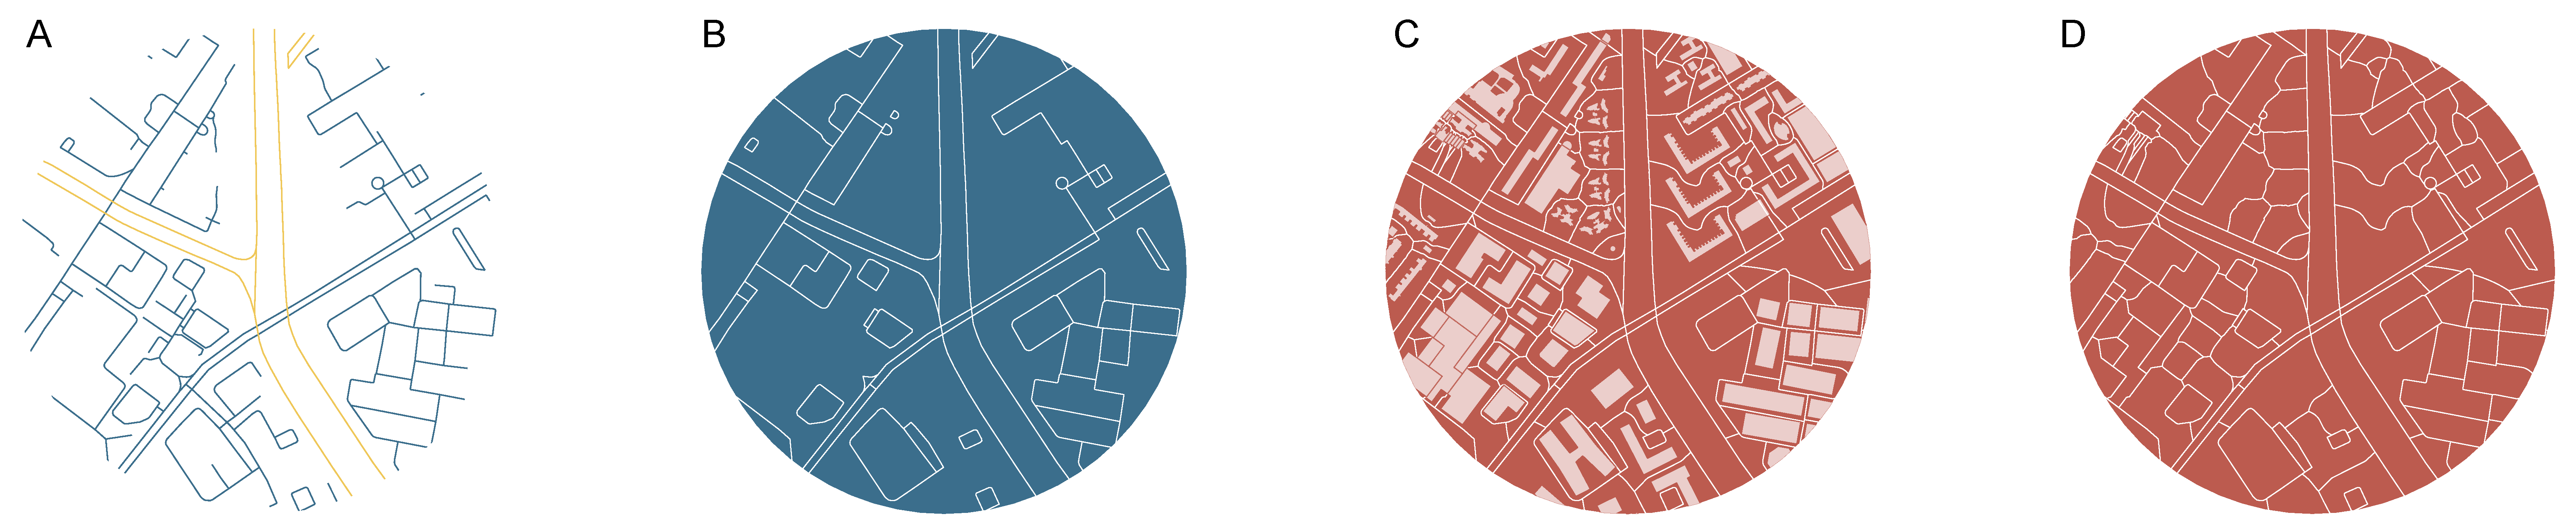
\includegraphics[width=\linewidth]{figures/et_diagram.pdf}
\caption{Diagram illustrating the sequential steps leading to the delineation of
enclosed tessellaion. From a series of enclosing components, where blue are streets and
yellow river banks (A), to enclosures (shown as blue polygons) (B),
incorporation of buildings as anchors (C) to final tessellation cells shown as red polygons (D).}
\label{fig:et_diagram}
\end{figure}


%%% Gather all enclosing features (streets, rivers, railways, etc.)
First, they rely on a set of enclosing components: features of the landscape
that divide it in smaller, fully delimited portions. The list of what should be
counted as enclosing is informed by theory and, as we will see below, may vary
by context. But, as an illustration, it includes elements such as the street
network, rivers and coastlines, or railways.
%%% Build enclosing geography
Second, these enclosing features are integrated into a single set of boundaries
that partition the geography into smaller areas. In some cases, they will be
small, as with urban blocks in dense city centres; in others, they will be
larger in size, as in rural sections with lower density of enclosing features.
We call each of this fully delimited areas an enclosure.
%%% subdivision it based on building presence
Third, enclosures are further subdivided using a morphological tesselation
\citep{fleischmann2020morphological}
that exhaustively partitions space based on a set of building footprints,
which are used in this context as anchors to draw catchment polygons.
%%
This process generates geographical boundaries for a given area that result in a
new spatial unit. This unit provides full geographical coverage without any
overlap.
%
Since the essence of the approach resides in growing a tessellation inside a set
of enclosing features, we call the resulting areas ``enclosed tesselation
cells''.

%% Two foundational blocks:
The enclosed tessellation (ET) intersects two perspectives of how space can be
understood and organised.
%
%%% Enclosures (delimitters)
The first relies on the use of features that \textit{delimit} the landscape and
partition it into smaller, fully enclosed portions. These include the road and
street networks, but also others such as railways or rivers. Each feature is
conceptualised as a line that acts as a boundary, dividing space into what falls
within each of its sides.
%
A long tradition in the literature on urban perception relies on
variations of these delimiters. Prominent
early examples include the edges and paths highlighted by \cite{lynch1960} as
two of the five core elements that define legibility and imageability of a city;
as well as the later work inspired by this framework (e.g. \citealp{filomena2019a}).

%%% Building (subdelimitters) --> use morphometric lit to justify why buildings
%are so relevant
The second perspective that ET integrate is a vision organised around
\textit{anchors}. In this view, space arises in-between
a discrete set of relevant features. Unlike delimiters, these elements do not
partition space per se, but instead act as origins to which the rest can be
``attached''.
%
The choice of anchors might vary by context but, in this case, the literature on
morphometrics has extensive evidence to support the use of buildings as the
primary feature \citep{hamaina2012a, usui2013estimation, schirmer2015}.

% [Build illustration in the description]

% Why --> meets every requirement and extends the previous state-of-the-art
The combination of delimiters and anchors as the parsers of space make ECs an
ideal spatial unit to study spatial signatures, one which
meets the three requirements we outlined above.
%
They are indivisable in that a single EC will contain no delimiters, at most a
single anchor, and potentially none.
%
They are also internally consistent because they are delineated as the area
within the delimiters that contain at most one anchor.
%
And finally ECs are exhaustive in that every location within the area of
interest is assigned to one and only one EC, providing full geographical
coverage without any overlap.


\subsection{Embedding form and function into Spatial Signatures}
\label{ssec:ss_ff}

% attaching data that relate to a cell to characterise it
% intrinsic char of cell
% other part of the context
% some relate to form
% some relate to function

% Section 4 - Empirics
\section{Illustration}
\label{sec:app}

% when talking about BCN mention
% https://www.researchgate.net/publication/254457523_Urban_form_and_compactness_of_morphological_homogeneous_districts_in_Barcelona_towards_an_automatic_classification_of_similar_built-up_structures_in_the_city#

% all technical details in to an appendix tables from excel should go to notebooks

\subsection{Method}
%%%%%%%%%%%% Structure 4.1 (squeeze it in a page) introduction of cases - 1 per
% continent; geographical variation, take different cities, cultures, historical moments

% spatial signature is a conceptual framework which can materialise in different ways
The classification of built form into spatial signatures is a conceptual framework and
as such, can materialise in different ways depending on the particular implementation of
a description of both form and function and the method of aggregation of enclosed cells
into singatures.
% here we present it applied to five cases from around the world
Here we present the concept applied to five case studies, reflecting different
environments and heterogeneous input data requiring the adaptation of the classification
to individual situations.
% the sample comes with geographical variation - 1, 2, 3, 4, 5
The sample offers a geographical variation covering Europe (Barcelona, Spain), North
America (Houston, TX, United States), South America (Medellin, Colombia), Africa (Dar es
Salaam, Tanzania) and South-east Asia (Singapore),
% that brings different culture, development, planning paradigm, historical and social
% contexts
coupled with cultural diversity, different planning paradigms involved in shaping the
respective environments as well as varied historical and social contexts in which the
selected cities were built.
% at the same time, it brings different input data, varied in both quality and richness
At the same time, the selection brings a variety of input data covering both extremes in
terms of quality (e.g., official mapping in Barcelona vs remote sensing in Houston), the
richness of information on functional aspects of places (e.g., detailed data on the
municipal level in Medellin vs global gridded datasets in Dar es Salaam) and scale
(82,375 units in Barcelona vs 2,043,581 units in Houston).
% we present this variety to illustrate the application and flexibility of the concept
We present this variety to illustrate the flexibility of spatial signatures to
accommodate varied inputs and adapt to a local specificity, while retaining the merit of
the concept.

%% method - top level outline of the method. Data, Form + convolution, Function,
% Clustering One para on how to build the data - F+F+Convolution, how it varies across
% examples (link to App.)

%%% shall we add conceptual diagram of the method?

% 1. data retrieval from open sources
The delineation of spatial signatures starts with the input data reflecting form and
function of each place. We use enclosed tessellation, outlined in the
\hyperref[sec:ssec:ss_et]{section 3.2}, as a basic spatial unit. Therefore, the input
data should consist of building footprints and physical barriers denoting streets,
railways, and water bodies.
% 2. geographies - enclosures, enclosed tessellation
Using barriers, we first identify the geometry of enclosures to determine the external
boundaries of consequently generated enclosed tessellation.
% 3. characterization of form - primary + convolutions
Resulting set of geometric data is rich enough for a comprehensive morphometric analysis
composed of primary measurable characters, capturing individual aspects of form, and
contextualisation, following the model proposed by
\citealp{fleischmann2021methodological}. In the contextualisation step, we measure the
tendencies of the distribution of each character within the neighbouring context of each
tessellation cell.
% 4. characterisation of function
Function is captured as a heterogeneous set of datasets reflecting aspects from
population to location of points of interest. All aspects are linked to enclosed cells
using the most appropriate method for each data input (e.g., areal interpolation or
network accessibility).\footnote{See the technical appendix for details on the
implementation.} The complete list of used characters relfecting both form and function
is available as an appendix XXX.

% Second para on how we generate signatures (clustering); once we have those we
% dissolve.

% 5. cluster analysis input (all linked to cell)
Spatial signatures are then identified using cluster analysis of tessellation cells
based on their form-function characteristics, combined with the notion of contiguity,
where each contiguous portion of land belonging to a single cluster is seen as a single
signature.
% 6. clustergram
The combined data reflecting both form and function are therefore standardised and
clustered using K-Means clustering. Since the number of classes is not known a priori,
we use clustergram \citep{schonlau2002clustergram} to understand clustering behaviour
within different options and select the optimal number according to its structure.
% 7. clustering
The final clustering is run with 1000 initialisations to ensure the stability of the
results.
% 8. dissolution
The geometry of each spatial signature is then derived as dissolution of a contiguous
patch of enclosed tessellation within the same cluster.


\subsection{Results}
% 4.2 (a page and a half) Results; tell some stories to get reader on board

%%% Para1 how to read the map in an applied way geometries reflect boundaries of spatial
% signatures
Figures XXX-YYY illustrate the resulting spatial signatures in the respective case
studies.\footnote{For intermediate steps (e.g. clustergram) please refer to the
technical appendix.} The geometries reflect the spatial extent of individual signatures
derived from the enclosed tessellation
% colours reflect a type of a signature - two areas within the same type share the
% characteristics; similarity of colours has no meaning
with colour coding reflecting the type of a signature, i.e. the initial cluster. Two
areas within the same type are expected to share the characteristics of built
environment, being more similar (not necessarily the same) to each other than to the
rest of the classes. Note that the similarity of different colours does not encode
similarity of signatures. Also note, that due to varied extent of case studies, maps are
not printed at the same scale.

%%% Para2 things which are shared/consistent 9-19 clusters, not dependent on the scale
% but reflecting the heterogeneity of a place
The granularity of classification ranges from 9 (Houston) to 19 (Medellin) signature
types per case study. However, the actual number is not dependent on the size of each
city but rather on each place's actual heterogeneity, best illustrated on the comparison
of Houston and Barcelona, the largest (2 million cells) and the smallest (80 thousand
cells) case. Houston, representing north American sprawling urban fabric shows a
considerably smaller diversity of spatial patterns (9 types of spatial signatures) than
Barcelona (16 types), reflecting the richness of their respective historical
developments.
% core clusters and outlier clusters - the abundance varies a lot
The distribution of cluster sizes follows the same pattern of unequal abundance across
all cases. The most extensive types contain between 15 and 28% of all
observations, and the abundance is gradually decreasing towards a small number of
outlier clusters containing less than a per cent of all observations within each sample.
% transition from core to countryside - singapore is exception, its island nature
% restricts such behaviour
All the cases clearly defined both extremes on the urbanisation axis, with delineated
central districts on the one hand and non-urban countryside signatures on the other. The
transition between the two tends to follow the gradual pattern of signatures each less
urban than the previous. The only exception where this tendency is not so profound (but
still present) is Singapore, which geographical extent limited to the defined area of
the main island does not allow the full transition.


%%% Para3 interesting stories from cases (BCN village centres, DeS slums) BCN reflects
% its historical origin - pre-industrial core and village centes, later filled by
% eixample, which has its homogenous core and areas blending into the existing fabric
Barcelona is known for its industrial grid, which is captured as a unique signature.
However, the Cerda’s grid is historically an infill between the city's medieval core and
smaller existing settlements around. Both core and former independent villages are
reflected in the typology of signatures, which reflect the historical origin of distinct
places. The transition between the two, the historical organic fabrics and rigid
Eixample is reflected as another signature, stitching together different patterns into a
coherent city.
% Medellin's change of the pattern as we go up the hill from the central valley
% - central plateu allows more rigid planning reflected in several classes, hillsides
%   are becoming more vernacular
Spatial distribution of signatures in Medellin tells the story of its intricate
topography, even though the input data do not contain any information on altitude. The
city lies in the valley surrounded by steep slopes. While the central parts lie on the
relatively flat floor allowing paradigmatic planning and rigidness of the built
environment, hillsides are becoming more vernacular leading to a sharp urban edge where
the topography does not allow further development.

% Dar es Salaam signatures capture different levels of formality, planned, semi-formal
% to informal
Signatures in Dar es Salaam reflect the changes in the formality of development, with
formal areas distributed in the central parts of the city in the vicinity of a
coastline. The transition between different degrees of formality is not always gradual
as the most informal parts of the city are infills of the space not occupied by more
planned neighbourhoods.

% houston and its homogenous sprawl, changing its nature of sprawlness along the time
% and growth, with major roads forming spines of non-residential development
The character of spatial signatures in Houston follows two primary principles. One type
forms the spine of activity spreading from the city centre radially to the suburbs. The
other, filling the areas in between the former, is a story of the deterioration of
compact, walkable urban block into convoluted dendritic street network patterns of
modern suburbs. The change in these predominantly residential signatures is gradual and
reflect the waves of development of the city as it was growing over the years.
% NOTE: Houston signatures are not able to distinguish CBD from the rest of the "spine",
% shall we dicuss that at some point?

% Singapore singature tell the story of its growth. we can follow individual clusters
% and link their origin to different time periods
A similar situation is in Singapore, where different types of signatures can be linked
to the period of the origin of the development of each specific neighbourhood. Contrary
to previous cases, the development and, consequently, spatial signatures followed radial
manner, not entirely contiguous, with major infills built in the last 50 years.


% Section 5 - Conclusion
\section{Conclusions} 
\label{sec:conclusions}



\clearpage




\bibliographystyle{apalike}
\bibliography{refs}

\clearpage

\appendix
\section{Technical appendix}
\label{sec:appendix}

\subsection{The complete lists of used characters relfecting both form and function across case studies}

\small
\begin{longtable}{p{5cm}p{4cm}p{4cm}l}
\caption{The complete list of form characters used in the Barcelona case study. The implementation details are available
in Jupyter notebooks available at <anonymised for peer-review>.}
\label{tab:form_bcn} \\
\toprule
                                   index &                         element &                    context &     category \\
\midrule
\endfirsthead

\toprule
                               index &                         element &                    context &     category \\
\midrule
\endhead
\midrule
\multicolumn{4}{r}{{Continued on next page}} \\
\midrule
\endfoot

\bottomrule
\endlastfoot
                                area &                        building &                   building &    dimension \\
                           perimeter &                        building &                   building &    dimension \\
                      courtyard area &                        building &                   building &    dimension \\
                circular compactness &                        building &                   building &        shape \\
                             corners &                        building &                   building &        shape \\
                          squareness &                        building &                   building &        shape \\
        equivalent rectangular index &                        building &                   building &        shape \\
                          elongation &                        building &                   building &        shape \\
centroid - corner distance deviation &                        building &                   building &        shape \\
     centroid - corner mean distance &                        building &                   building &    dimension \\
                   solar orientation &                        building &                   building & distribution \\
                    street alignment &                        building &                   building & distribution \\
                      cell alignment &                        building &                   building & distribution \\
                 longest axis length &               tessellation cell &          tessellation cell &    dimension \\
                                area &               tessellation cell &          tessellation cell &    dimension \\
                circular compactness &               tessellation cell &          tessellation cell &        shape \\
        equivalent rectangular index &               tessellation cell &          tessellation cell &        shape \\
                   solar orientation &               tessellation cell &          tessellation cell & distribution \\
                 coverage area ratio &               tessellation cell &          tessellation cell &    intensity \\
                    street alignment &               tessellation cell &          tessellation cell & distribution \\
                              length &                  street segment &             street segment &    dimension \\
                               width &                  street profile &             street segment &    dimension \\
                            openness &                  street profile &             street segment & distribution \\
                     width deviation &                  street profile &             street segment &    diversity \\
                           linearity &                  street segment &             street segment &        shape \\
                        area covered &                  street segment &             street segment &    dimension \\
                 buildings per meter &                  street segment &             street segment &    intensity \\
                        area covered &                     street node &                street node &    dimension \\
                           alignment &          neighbouring buildings & neighbouring cells (queen) & distribution \\
                       mean distance &          neighbouring buildings & neighbouring cells (queen) & distribution \\
                 weighted neighbours &               tessellation cell & neighbouring cells (queen) & distribution \\
                        area covered &              neighbouring cells & neighbouring cells (queen) &    dimension \\
                        reached area &           neighbouring segments &      neighbouring segments &    dimension \\
                       reached cells &           neighbouring segments &      neighbouring segments &    intensity \\
                              degree &                     street node &         neighbouring nodes & distribution \\
 mean distance to neighbouring nodes &                     street node &         neighbouring nodes &    dimension \\
                  shared walls ratio &             adjacent buildings  &        adjacent buildings  & distribution \\
        mean inter-building distance &          neighbouring buildings &    cell queen neighbours 3 & distribution \\
         weighted reached enclosures & neighbouring tessellation cells &    cell queen neighbours 3 &    intensity \\
                                area &                       enclosure &                  enclosure &    dimension \\
                           perimeter &                       enclosure &                  enclosure &    dimension \\
                circular compactness &                       enclosure &                  enclosure &        shape \\
        equivalent rectangular index &                       enclosure &                  enclosure &        shape \\
           compactness-weighted axis &                       enclosure &                  enclosure &        shape \\
                   solar orientation &                       enclosure &                  enclosure & distribution \\
                 weighted neighbours &                       enclosure &                  enclosure & distribution \\
                      weighted cells &                       enclosure &                  enclosure &    intensity \\
                    local meshedness &                  street network &              nodes 5 steps & connectivity \\
                 mean segment length &                  street network &            segment 3 steps &    dimension \\
                   cul-de-sac length &                  street network &              nodes 3 steps &    dimension \\
                        node density &                  street network &              nodes 5 steps &    intensity \\
           proportion of cul-de-sacs &                  street network &              nodes 5 steps & connectivity \\
   proportion of 3-way intersections &                  street network &              nodes 5 steps & connectivity \\
   proportion of 4-way intersections &                  street network &              nodes 5 steps & connectivity \\
        degree weighted node density &                  street network &              nodes 5 steps &    intensity \\
          local closeness centrality &                  street network &              nodes 5 steps & connectivity \\
               perimeter wall length &             adjacent buildings  &           joined buildings &    dimension \\
                number of courtyards &             adjacent buildings  &           joined buildings &    intensity \\
                   square clustering &                  street network &             street network & connectivity \\
\end{longtable}


\begin{longtable}{p{5cm}p{3cm}p{5cm}}
\caption{The complete list of function characters and transfer methods used in the Barcelona case study. The implementation details are available
in Jupyter notebooks available at <anonymised for peer-review>.}
\label{tab:fn_bcn} \\
\toprule
                                         character & input spatial unit &                                    transfer method \\
\midrule
\endfirsthead

\toprule
                                         character & input spatial unit &                                    transfer method \\
\midrule
\endhead
\midrule
\multicolumn{3}{r}{{Continued on next page}} \\
\midrule
\endfoot

\bottomrule
\endlastfoot
                                        population &              block &                  Building-based Dasymetric mapping \\
                               number of car parks &              block &                                 Dasymetric mapping \\
       number of other items that are not premises &              block &                                 Dasymetric mapping \\
                                          land use &             parcel &                            Spatial join (centroid) \\
                               number of dwellings &           building &                                     Attribute join \\
                                       current use &           building &                                     Attribute join \\
                                               age &           building &                                     Attribute join \\
                                          heritage &             points &                     Accessibility  -\# within 15min \\
                                          heritage &           polygons &                                       Spatial join \\
   culture (cinemas, museums, libraries, theaters) &             points & Accessibility  - distance to nearest / \# within 15min \\
                                             parks &             points & Accessibility  - distance to nearest / \# within 15min \\
                                   economic census &            poitnts & Accessibility  - distance to nearest / \# within 15min \\
                                       restaurants &              point & Accessibility  - distance to nearest / \# within 15min \\
                                             trees &             points &                               Spatial join (count) \\
                                              NDVI &          raster 1m &                                        Zonal stats \\
\end{longtable}

\begin{longtable}{p{5cm}p{4cm}p{4cm}l}
\caption{The complete list of form characters used in the BarceMedellinlona case study. The implementation details are available
in Jupyter notebooks available at <anonymised for peer-review>.}
\label{tab:form_med} \\
\toprule
                                index &                         element &                    context &     category \\
\midrule
\endfirsthead

\toprule
                                index &                         element &                    context &     category \\
\midrule
\endhead
\midrule
\multicolumn{4}{r}{{Continued on next page}} \\
\midrule
\endfoot

\bottomrule
\endlastfoot
                                area &                        building &                   building &    dimension \\
                            perimeter &                        building &                   building &    dimension \\
                        courtyard area &                        building &                   building &    dimension \\
                circular compactness &                        building &                   building &        shape \\
                                corners &                        building &                   building &        shape \\
                            squareness &                        building &                   building &        shape \\
        equivalent rectangular index &                        building &                   building &        shape \\
                            elongation &                        building &                   building &        shape \\
centroid - corner distance deviation &                        building &                   building &        shape \\
        centroid - corner mean distance &                        building &                   building &    dimension \\
                    solar orientation &                        building &                   building & distribution \\
                    street alignment &                        building &                   building & distribution \\
                        cell alignment &                        building &                   building & distribution \\
                    longest axis length &               tessellation cell &          tessellation cell &    dimension \\
                                area &               tessellation cell &          tessellation cell &    dimension \\
                circular compactness &               tessellation cell &          tessellation cell &        shape \\
        equivalent rectangular index &               tessellation cell &          tessellation cell &        shape \\
                    solar orientation &               tessellation cell &          tessellation cell & distribution \\
                    coverage area ratio &               tessellation cell &          tessellation cell &    intensity \\
                    street alignment &               tessellation cell &          tessellation cell & distribution \\
                                length &                  street segment &             street segment &    dimension \\
                                width &                  street profile &             street segment &    dimension \\
                            openness &                  street profile &             street segment & distribution \\
                        width deviation &                  street profile &             street segment &    diversity \\
                            linearity &                  street segment &             street segment &        shape \\
                        area covered &                  street segment &             street segment &    dimension \\
                    buildings per meter &                  street segment &             street segment &    intensity \\
                        area covered &                     street node &                street node &    dimension \\
                            alignment &          neighbouring buildings & neighbouring cells (queen) & distribution \\
                        mean distance &          neighbouring buildings & neighbouring cells (queen) & distribution \\
                    weighted neighbours &               tessellation cell & neighbouring cells (queen) & distribution \\
                        area covered &              neighbouring cells & neighbouring cells (queen) &    dimension \\
                        reached area &           neighbouring segments &      neighbouring segments &    dimension \\
                        reached cells &           neighbouring segments &      neighbouring segments &    intensity \\
                                degree &                     street node &         neighbouring nodes & distribution \\
    mean distance to neighbouring nodes &                     street node &         neighbouring nodes &    dimension \\
                    shared walls ratio &             adjacent buildings  &        adjacent buildings  & distribution \\
        mean inter-building distance &          neighbouring buildings &    cell queen neighbours 3 & distribution \\
            weighted reached enclosures & neighbouring tessellation cells &    cell queen neighbours 3 &    intensity \\
                                area &                       enclosure &                  enclosure &    dimension \\
                            perimeter &                       enclosure &                  enclosure &    dimension \\
                circular compactness &                       enclosure &                  enclosure &        shape \\
        equivalent rectangular index &                       enclosure &                  enclosure &        shape \\
            compactness-weighted axis &                       enclosure &                  enclosure &        shape \\
                    solar orientation &                       enclosure &                  enclosure & distribution \\
                    weighted neighbours &                       enclosure &                  enclosure & distribution \\
                        weighted cells &                       enclosure &                  enclosure &    intensity \\
                    local meshedness &                  street network &              nodes 5 steps & connectivity \\
                    mean segment length &                  street network &            segment 3 steps &    dimension \\
                    cul-de-sac length &                  street network &              nodes 3 steps &    dimension \\
                        node density &                  street network &              nodes 5 steps &    intensity \\
            proportion of cul-de-sacs &                  street network &              nodes 5 steps & connectivity \\
    proportion of 3-way intersections &                  street network &              nodes 5 steps & connectivity \\
    proportion of 4-way intersections &                  street network &              nodes 5 steps & connectivity \\
        degree weighted node density &                  street network &              nodes 5 steps &    intensity \\
            local closeness centrality &                  street network &              nodes 5 steps & connectivity \\
                perimeter wall length &             adjacent buildings  &           joined buildings &    dimension \\
                number of courtyards &             adjacent buildings  &           joined buildings &    intensity \\
                    square clustering &                  street network &             street network & connectivity \\
\end{longtable}


\begin{longtable}{p{5cm}p{3cm}p{5cm}}
\caption{The complete list of function characters and transfer methods used in the Medellin case study. The implementation details are available
in Jupyter notebooks available at <anonymised for peer-review>.}
\label{tab:fn_med} \\
\toprule
                                            character & input spatial unit &                                    transfer method \\
\midrule
\endfirsthead

\toprule
                                            character & input spatial unit &                                    transfer method \\
\midrule
\endhead
\midrule
\multicolumn{3}{r}{{Continued on next page}} \\
\midrule
\endfoot

\bottomrule
\endlastfoot
                trees &   points &                               Spatial join (count) \\
                parks & polygons &                                Distance to nearest \\
heritage large areas & polygons &                               Spatial join (boolean) \\
            land use & polygons &                                             tobler \\
                pois &   points & Accessibility  - distance to nearest / \# within 15min \\
        public spaces & polygons &             Accessibility  -  area within radius \\
            population &   raster &                                        Zonal stats \\
                NDVI &   raster &                                        Zonal stats \\
\end{longtable}


\begin{longtable}{p{5cm}p{4cm}p{4cm}l}
    \caption{The complete list of form characters used in the Dar es Salaam case study. The implementation details are available
    in Jupyter notebooks available at <anonymised for peer-review>.}
    \label{tab:form_des} \\
    \toprule
                                   index &                         element &                    context &     category \\
    \midrule
    \endfirsthead

    \toprule
                                   index &                         element &                    context &     category \\
    \midrule
    \endhead
    \midrule
    \multicolumn{4}{r}{{Continued on next page}} \\
    \midrule
    \endfoot

    \bottomrule
    \endlastfoot
                                    area &                        building &                   building &    dimension \\
                               perimeter &                        building &                   building &    dimension \\
                          courtyard area &                        building &                   building &    dimension \\
                    circular compactness &                        building &                   building &        shape \\
                                 corners &                        building &                   building &        shape \\
                              squareness &                        building &                   building &        shape \\
            equivalent rectangular index &                        building &                   building &        shape \\
                              elongation &                        building &                   building &        shape \\
    centroid - corner distance deviation &                        building &                   building &        shape \\
         centroid - corner mean distance &                        building &                   building &    dimension \\
                       solar orientation &                        building &                   building & distribution \\
                        street alignment &                        building &                   building & distribution \\
                          cell alignment &                        building &                   building & distribution \\
                     longest axis length &               tessellation cell &          tessellation cell &    dimension \\
                                    area &               tessellation cell &          tessellation cell &    dimension \\
                    circular compactness &               tessellation cell &          tessellation cell &        shape \\
            equivalent rectangular index &               tessellation cell &          tessellation cell &        shape \\
                       solar orientation &               tessellation cell &          tessellation cell & distribution \\
                     coverage area ratio &               tessellation cell &          tessellation cell &    intensity \\
                                  length &                  street segment &             street segment &    dimension \\
                                   width &                  street profile &             street segment &    dimension \\
                                openness &                  street profile &             street segment & distribution \\
                         width deviation &                  street profile &             street segment &    diversity \\
                               linearity &                  street segment &             street segment &        shape \\
                            area covered &                  street segment &             street segment &    dimension \\
                     buildings per meter &                  street segment &             street segment &    intensity \\
                            area covered &                     street node &                street node &    dimension \\
                               alignment &          neighbouring buildings & neighbouring cells (queen) & distribution \\
                           mean distance &          neighbouring buildings & neighbouring cells (queen) & distribution \\
                     weighted neighbours &               tessellation cell & neighbouring cells (queen) & distribution \\
                            area covered &              neighbouring cells & neighbouring cells (queen) &    dimension \\
                           reached cells &           neighbouring segments &      neighbouring segments &    intensity \\
                            reached area &           neighbouring segments &      neighbouring segments &    dimension \\
                                  degree &                     street node &         neighbouring nodes & distribution \\
     mean distance to neighbouring nodes &                     street node &         neighbouring nodes &    dimension \\
            mean inter-building distance &          neighbouring buildings &    cell queen neighbours 3 & distribution \\
             weighted reached enclosures & neighbouring tessellation cells &    cell queen neighbours 3 &    intensity \\
                       reached neighbors & neighbouring tessellation cells &    cell queen neighbours 3 &    intensity \\
                            reached area & neighbouring tessellation cells &    cell queen neighbours 3 &    dimension \\
                                    area &                       enclosure &                  enclosure &    dimension \\
                               perimeter &                       enclosure &                  enclosure &    dimension \\
                    circular compactness &                       enclosure &                  enclosure &        shape \\
            equivalent rectangular index &                       enclosure &                  enclosure &        shape \\
               compactness-weighted axis &                       enclosure &                  enclosure &        shape \\
                       solar orientation &                       enclosure &                  enclosure & distribution \\
                     weighted neighbours &                       enclosure &                  enclosure & distribution \\
                          weighted cells &                       enclosure &                  enclosure &    intensity \\
                        local meshedness &                  street network &              nodes 5 steps & connectivity \\
                     mean segment length &                  street network &            segment 3 steps &    dimension \\
                       cul-de-sac length &                  street network &              nodes 3 steps &    dimension \\
                            reached area &                  street network &            segment 3 steps &    dimension \\
                           reached cells &                  street network &            segment 3 steps &    intensity \\
                            node density &                  street network &              nodes 5 steps &    intensity \\
               proportion of cul-de-sacs &                  street network &              nodes 5 steps & connectivity \\
       proportion of 3-way intersections &                  street network &              nodes 5 steps & connectivity \\
       proportion of 4-way intersections &                  street network &              nodes 5 steps & connectivity \\
            degree weighted node density &                  street network &              nodes 5 steps &    intensity \\
              local closeness centrality &                  street network &              nodes 5 steps & connectivity \\
                       square clustering &                  street network &             street network & connectivity \\
\end{longtable}


\begin{longtable}{p{5cm}p{3cm}p{5cm}}
    \caption{The complete list of function characters and transfer methods used in the Dar es Salaam case study. The implementation details are available
    in Jupyter notebooks available at <anonymised for peer-review>.}
    \label{tab:fn_des} \\
    \toprule
                                             character & input spatial unit &                                    transfer method \\
    \midrule
    \endfirsthead

    \toprule
                                             character & input spatial unit &                                    transfer method \\
    \midrule
    \endhead
    \midrule
    \multicolumn{3}{r}{{Continued on next page}} \\
    \midrule
    \endfoot

    \bottomrule
    \endlastfoot
    population & raster 100m &     Zonal stats \\
          NDVI &  raster 10m &     Zonal stats \\
    land cover &      raster &     Zonal stats \\
  night lights &      raster &     Zonal stats \\
\end{longtable}


\begin{longtable}{p{5cm}p{4cm}p{4cm}l}
    \caption{The complete list of form characters used in the Houston case study. The implementation details are available
    in Jupyter notebooks available at <anonymised for peer-review>.}
    \label{tab:form_hou} \\
    \toprule
                                   index &                         element &                    context &     category \\
    \midrule
    \endfirsthead

    \toprule
                                   index &                         element &                    context &     category \\
    \midrule
    \endhead
    \midrule
    \multicolumn{4}{r}{{Continued on next page}} \\
    \midrule
    \endfoot

    \bottomrule
    \endlastfoot
                                    area &                        building &                   building &    dimension \\
                               perimeter &                        building &                   building &    dimension \\
                          courtyard area &                        building &                   building &    dimension \\
                    circular compactness &                        building &                   building &        shape \\
                                 corners &                        building &                   building &        shape \\
                              squareness &                        building &                   building &        shape \\
            equivalent rectangular index &                        building &                   building &        shape \\
                              elongation &                        building &                   building &        shape \\
    centroid - corner distance deviation &                        building &                   building &        shape \\
         centroid - corner mean distance &                        building &                   building &    dimension \\
                       solar orientation &                        building &                   building & distribution \\
                        street alignment &                        building &                   building & distribution \\
                          cell alignment &                        building &                   building & distribution \\
                     longest axis length &               tessellation cell &          tessellation cell &    dimension \\
                                    area &               tessellation cell &          tessellation cell &    dimension \\
                    circular compactness &               tessellation cell &          tessellation cell &        shape \\
            equivalent rectangular index &               tessellation cell &          tessellation cell &        shape \\
                       solar orientation &               tessellation cell &          tessellation cell & distribution \\
                     coverage area ratio &               tessellation cell &          tessellation cell &    intensity \\
                                  length &                  street segment &             street segment &    dimension \\
                                   width &                  street profile &             street segment &    dimension \\
                                openness &                  street profile &             street segment & distribution \\
                         width deviation &                  street profile &             street segment &    diversity \\
                               linearity &                  street segment &             street segment &        shape \\
                            area covered &                  street segment &             street segment &    dimension \\
                     buildings per meter &                  street segment &             street segment &    intensity \\
                               alignment &          neighbouring buildings & neighbouring cells (queen) & distribution \\
                           mean distance &          neighbouring buildings & neighbouring cells (queen) & distribution \\
                     weighted neighbours &               tessellation cell & neighbouring cells (queen) & distribution \\
                            area covered &              neighbouring cells & neighbouring cells (queen) &    dimension \\
                           reached cells &           neighbouring segments &      neighbouring segments &    intensity \\
                            reached area &           neighbouring segments &      neighbouring segments &    dimension \\
                                  degree &                     street node &         neighbouring nodes & distribution \\
     mean distance to neighbouring nodes &                     street node &         neighbouring nodes &    dimension \\
            mean inter-building distance &          neighbouring buildings &    cell queen neighbours 3 & distribution \\
             weighted reached enclosures & neighbouring tessellation cells &    cell queen neighbours 3 &    intensity \\
                       reached neighbors & neighbouring tessellation cells &    cell queen neighbours 3 &    intensity \\
                            reached area & neighbouring tessellation cells &    cell queen neighbours 3 &    dimension \\
                                    area &                       enclosure &                  enclosure &    dimension \\
                               perimeter &                       enclosure &                  enclosure &    dimension \\
                    circular compactness &                       enclosure &                  enclosure &        shape \\
            equivalent rectangular index &                       enclosure &                  enclosure &        shape \\
               compactness-weighted axis &                       enclosure &                  enclosure &        shape \\
                       solar orientation &                       enclosure &                  enclosure & distribution \\
                     weighted neighbours &                       enclosure &                  enclosure & distribution \\
                          weighted cells &                       enclosure &                  enclosure &    intensity \\
                        local meshedness &                  street network &              nodes 5 steps & connectivity \\
                     mean segment length &                  street network &            segment 3 steps &    dimension \\
                       cul-de-sac length &                  street network &              nodes 3 steps &    dimension \\
                            reached area &                  street network &            segment 3 steps &    dimension \\
                           reached cells &                  street network &            segment 3 steps &    intensity \\
                            node density &                  street network &              nodes 5 steps &    intensity \\
               proportion of cul-de-sacs &                  street network &              nodes 5 steps & connectivity \\
       proportion of 3-way intersections &                  street network &              nodes 5 steps & connectivity \\
       proportion of 4-way intersections &                  street network &              nodes 5 steps & connectivity \\
            degree weighted node density &                  street network &              nodes 5 steps &    intensity \\
              local closeness centrality &                  street network &              nodes 5 steps & connectivity \\
                       square clustering &                  street network &             street network & connectivity \\
\end{longtable}

\begin{longtable}{p{5cm}p{3cm}p{5cm}}
    \caption{The complete list of function characters and transfer methods used in the Houston case study. The implementation details are available
    in Jupyter notebooks available at <anonymised for peer-review>.}
    \label{tab:fn_hou} \\
    \toprule
                                             character & input spatial unit &                                    transfer method \\
    \midrule
    \endfirsthead

    \toprule
                                             character & input spatial unit &                                    transfer method \\
    \midrule
    \endhead
    \midrule
    \multicolumn{3}{r}{{Continued on next page}} \\
    \midrule
    \endfoot

    \bottomrule
    \endlastfoot
    population &  raster 100m &              Zonal stats \\
          NDVI &   raster 10m &              Zonal stats \\
    land cover &       raster &              Zonal stats \\
  night lights &       raster &              Zonal stats \\
    employment & census block & Dasymetric interpolation \\
historical sites &        point &            Accessibility \\
\end{longtable}


\begin{longtable}{p{5cm}p{4cm}p{4cm}l}
    \caption{The complete list of form characters used in the Singapore case study. The implementation details are available
    in Jupyter notebooks available at <anonymised for peer-review>.}
    \label{tab:form_sin} \\
    \toprule
                                   index &                         element &                    context &     category \\
    \midrule
    \endfirsthead

    \toprule
                                   index &                         element &                    context &     category \\
    \midrule
    \endhead
    \midrule
    \multicolumn{4}{r}{{Continued on next page}} \\
    \midrule
    \endfoot

    \bottomrule
    \endlastfoot
                                    area &                        building &                   building &    dimension \\
                               perimeter &                        building &                   building &    dimension \\
                          courtyard area &                        building &                   building &    dimension \\
                    circular compactness &                        building &                   building &        shape \\
                                 corners &                        building &                   building &        shape \\
                              squareness &                        building &                   building &        shape \\
            equivalent rectangular index &                        building &                   building &        shape \\
                              elongation &                        building &                   building &        shape \\
    centroid - corner distance deviation &                        building &                   building &        shape \\
         centroid - corner mean distance &                        building &                   building &    dimension \\
                       solar orientation &                        building &                   building & distribution \\
                        street alignment &                        building &                   building & distribution \\
                          cell alignment &                        building &                   building & distribution \\
                     longest axis length &               tessellation cell &          tessellation cell &    dimension \\
                                    area &               tessellation cell &          tessellation cell &    dimension \\
                    circular compactness &               tessellation cell &          tessellation cell &        shape \\
            equivalent rectangular index &               tessellation cell &          tessellation cell &        shape \\
                       solar orientation &               tessellation cell &          tessellation cell & distribution \\
                     coverage area ratio &               tessellation cell &          tessellation cell &    intensity \\
                        street alignment &               tessellation cell &          tessellation cell & distribution \\
                                  length &                  street segment &             street segment &    dimension \\
                                   width &                  street profile &             street segment &    dimension \\
                                openness &                  street profile &             street segment & distribution \\
                         width deviation &                  street profile &             street segment &    diversity \\
                               linearity &                  street segment &             street segment &        shape \\
                            area covered &                  street segment &             street segment &    dimension \\
                     buildings per meter &                  street segment &             street segment &    intensity \\
                            area covered &                     street node &                street node &    dimension \\
                               alignment &          neighbouring buildings & neighbouring cells (queen) & distribution \\
                           mean distance &          neighbouring buildings & neighbouring cells (queen) & distribution \\
                     weighted neighbours &               tessellation cell & neighbouring cells (queen) & distribution \\
                            area covered &              neighbouring cells & neighbouring cells (queen) &    dimension \\
                            reached area &           neighbouring segments &      neighbouring segments &    dimension \\
                           reached cells &           neighbouring segments &      neighbouring segments &    intensity \\
                                  degree &                     street node &         neighbouring nodes & distribution \\
     mean distance to neighbouring nodes &                     street node &         neighbouring nodes &    dimension \\
                      shared walls ratio &             adjacent buildings  &        adjacent buildings  & distribution \\
            mean inter-building distance &          neighbouring buildings &    cell queen neighbours 3 & distribution \\
             weighted reached enclosures & neighbouring tessellation cells &    cell queen neighbours 3 &    intensity \\
                                    area &                       enclosure &                  enclosure &    dimension \\
                               perimeter &                       enclosure &                  enclosure &    dimension \\
                    circular compactness &                       enclosure &                  enclosure &        shape \\
            equivalent rectangular index &                       enclosure &                  enclosure &        shape \\
               compactness-weighted axis &                       enclosure &                  enclosure &        shape \\
                       solar orientation &                       enclosure &                  enclosure & distribution \\
                     weighted neighbours &                       enclosure &                  enclosure & distribution \\
                          weighted cells &                       enclosure &                  enclosure &    intensity \\
                        local meshedness &                  street network &              nodes 5 steps & connectivity \\
                     mean segment length &                  street network &            segment 3 steps &    dimension \\
                       cul-de-sac length &                  street network &              nodes 3 steps &    dimension \\
                            node density &                  street network &              nodes 5 steps &    intensity \\
               proportion of cul-de-sacs &                  street network &              nodes 5 steps & connectivity \\
       proportion of 3-way intersections &                  street network &              nodes 5 steps & connectivity \\
       proportion of 4-way intersections &                  street network &              nodes 5 steps & connectivity \\
            degree weighted node density &                  street network &              nodes 5 steps &    intensity \\
              local closeness centrality &                  street network &              nodes 5 steps & connectivity \\
                   perimeter wall length &             adjacent buildings  &           joined buildings &    dimension \\
                    number of courtyards &             adjacent buildings  &           joined buildings &    intensity \\
                       square clustering &                  street network &             street network & connectivity \\
    \end{longtable}

\begin{longtable}{p{5cm}p{3cm}p{5cm}}
    \caption{The complete list of function characters and transfer methods used in the Singapore case study. The implementation details are available
    in Jupyter notebooks available at <anonymised for peer-review>.}
    \label{tab:fn_sin} \\
    \toprule
                                                character & input spatial unit &                                    transfer method \\
    \midrule
    \endfirsthead

    \toprule
                                                character & input spatial unit &                                    transfer method \\
    \midrule
    \endhead
    \midrule
    \multicolumn{3}{r}{{Continued on next page}} \\
    \midrule
    \endfoot

    \bottomrule
    \endlastfoot
    NDVI &  raster &         Zonal stats \\
population &  raster &         Zonal stats \\
night lights &  raster &         Zonal stats \\
eating est &   point &       Accessibility \\
supermarkets &   point &       Accessibility \\
land use & polygon & Areal interpolation \\
   parks &   point &       Accessibility \\
monuments &   point &       Accessibility \\
\end{longtable}

\normalsize

\subsection{Clustergrams}

\begin{figure}
    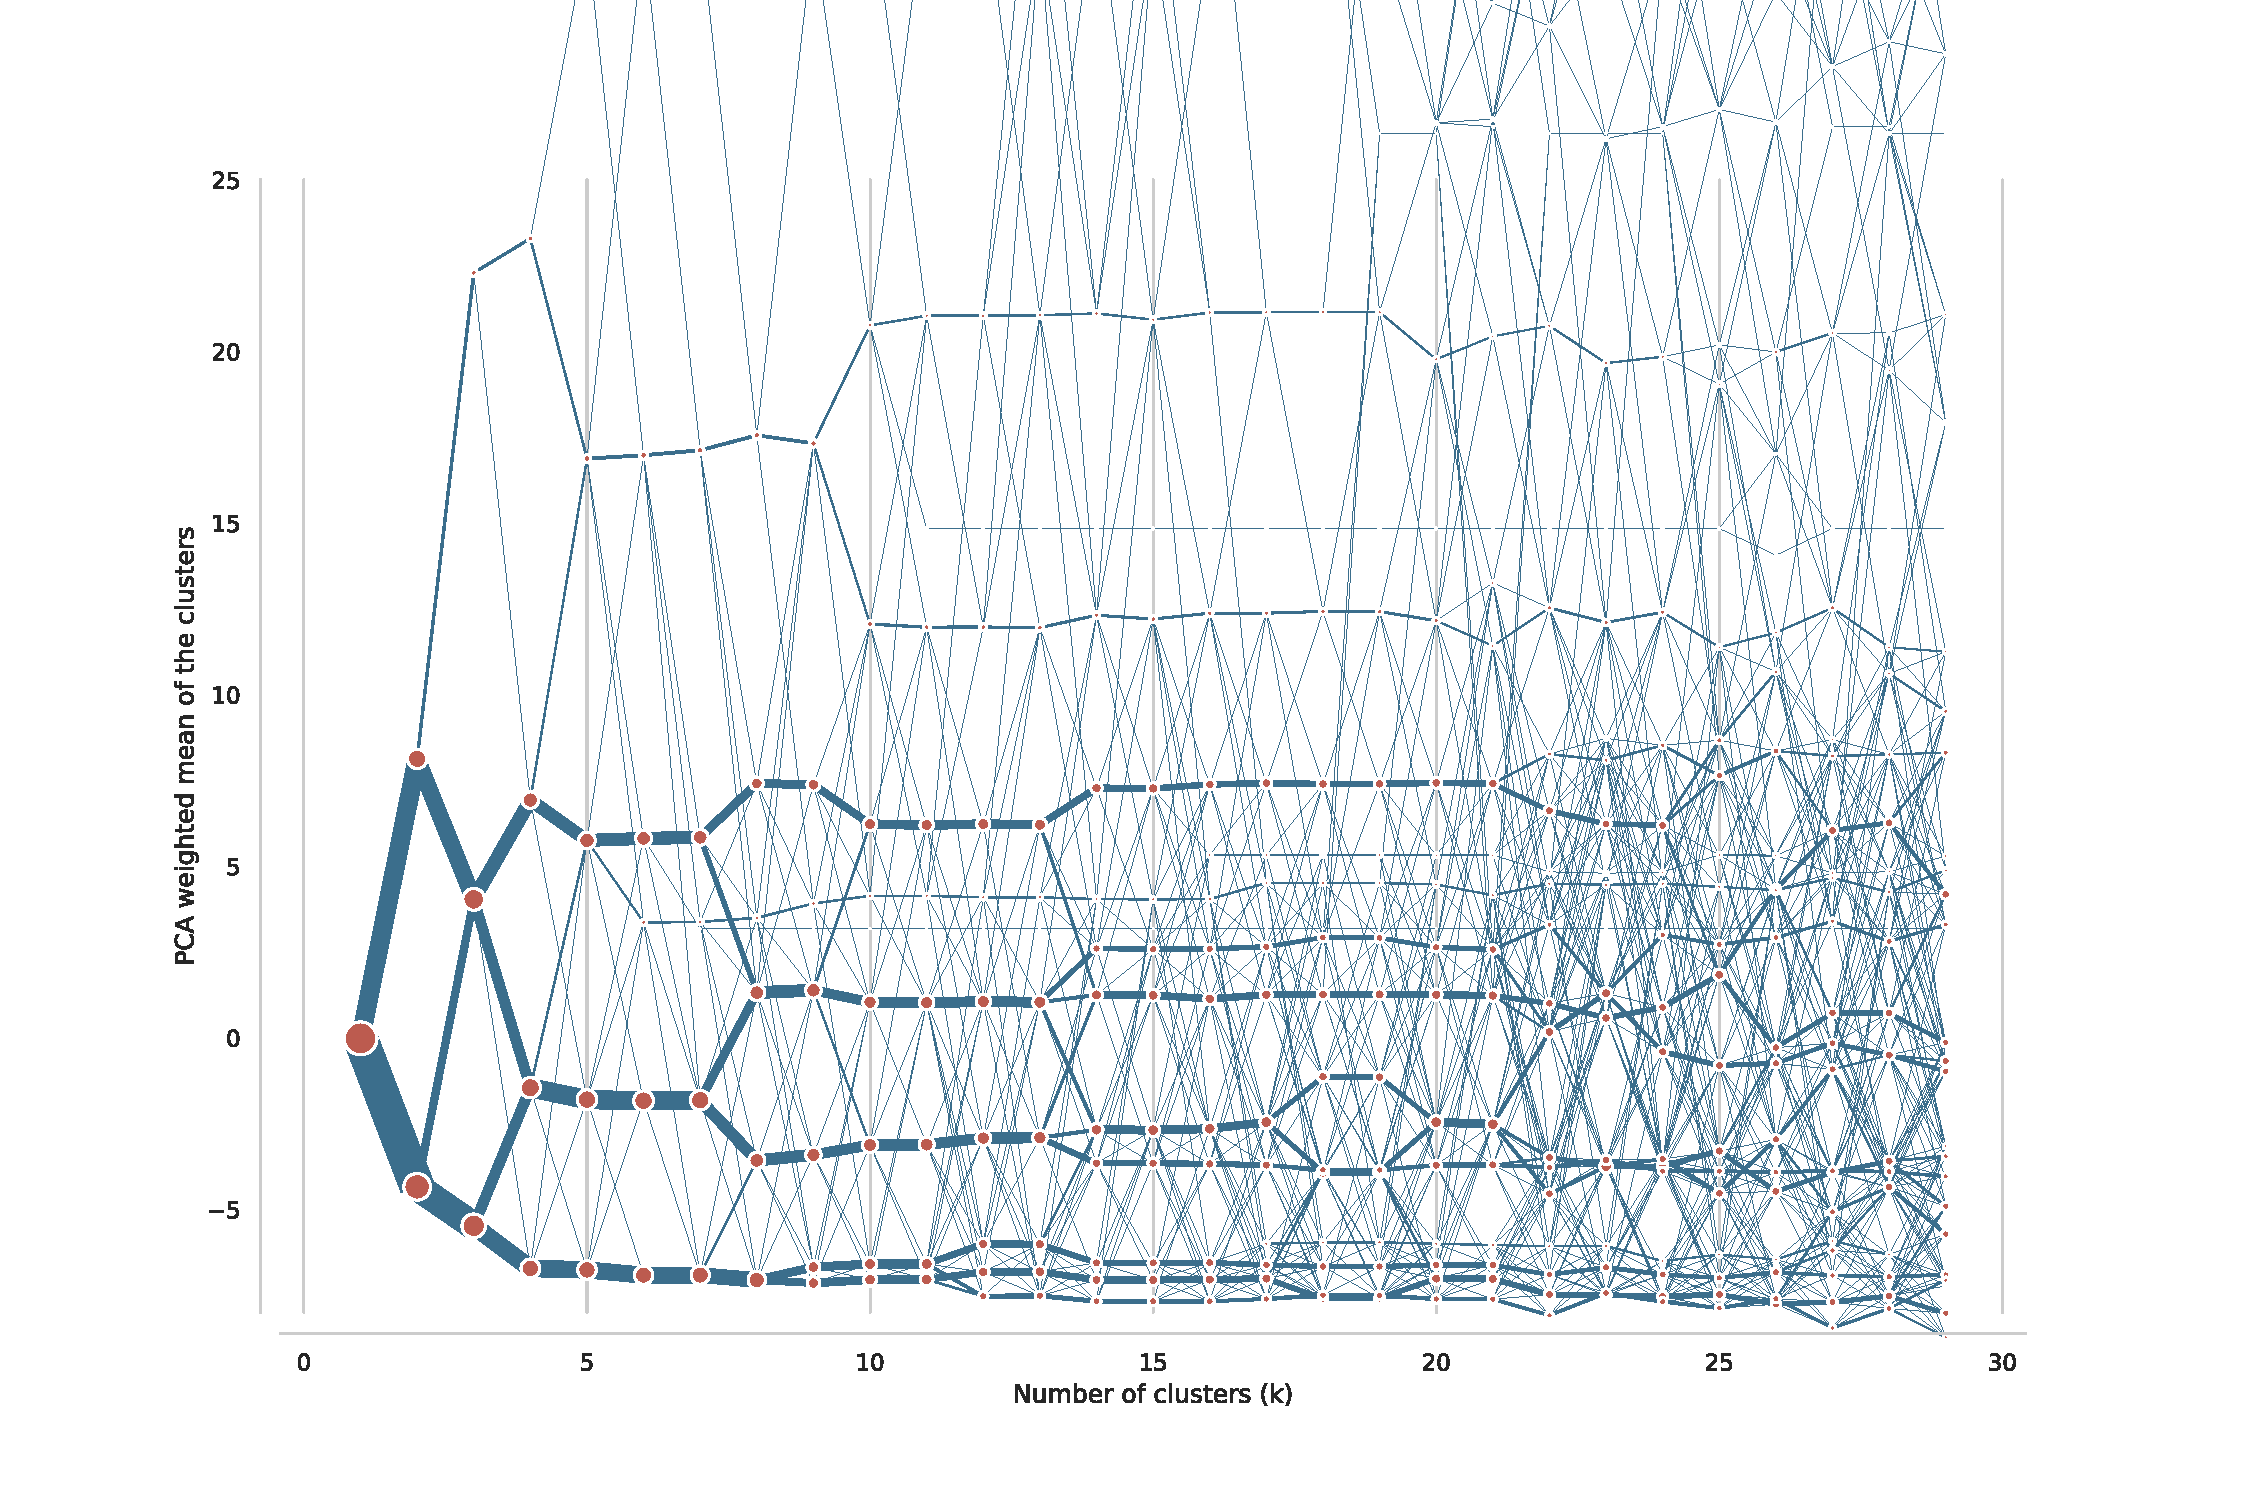
\includegraphics[width=\linewidth]{figures/clustergram_bcn.pdf}
    \caption{Clustergram (truncated along the vertical axis) illustrating the behaviour of dataset in different clustering options. The optimal number of clusters derived using the clustergram is 16.}
    \label{fig:cgram_bcn}
\end{figure}

\begin{figure}
    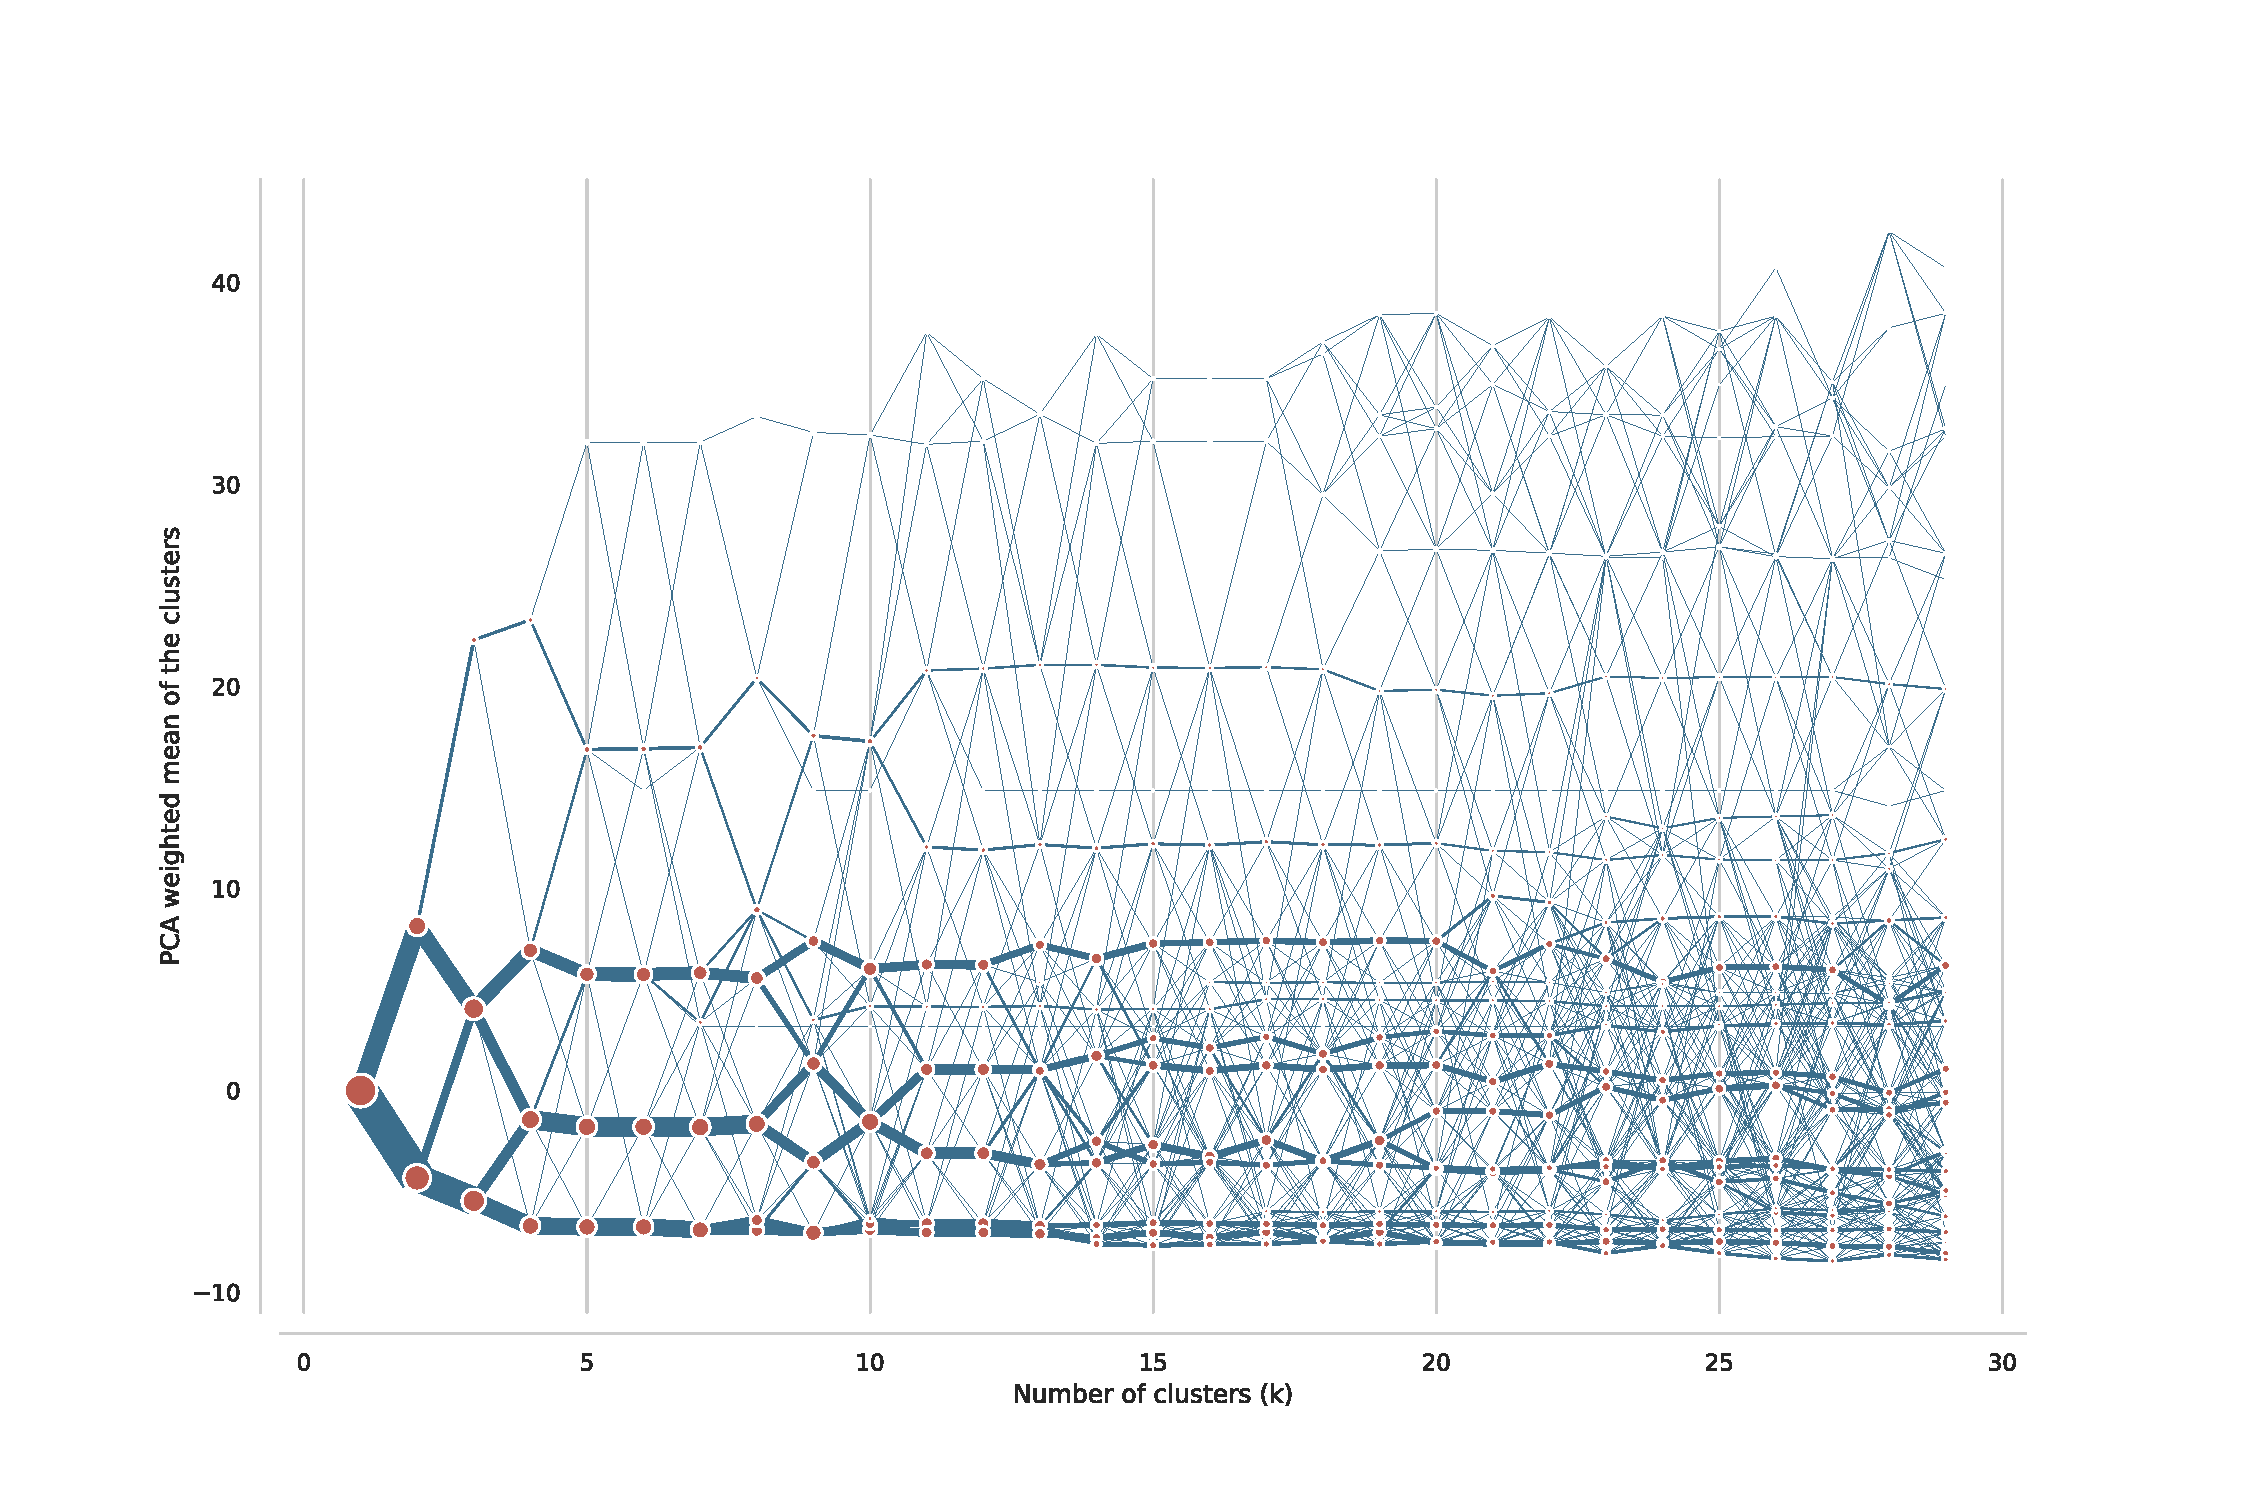
\includegraphics[width=\linewidth]{figures/clustergram_med.pdf}
    \caption{Clustergram (truncated along the vertical axis) illustrating the behaviour of dataset in different clustering options. The optimal number of clusters derived using the clustergram is 19.}
    \label{fig:cgram_med}
\end{figure}

\begin{figure}
    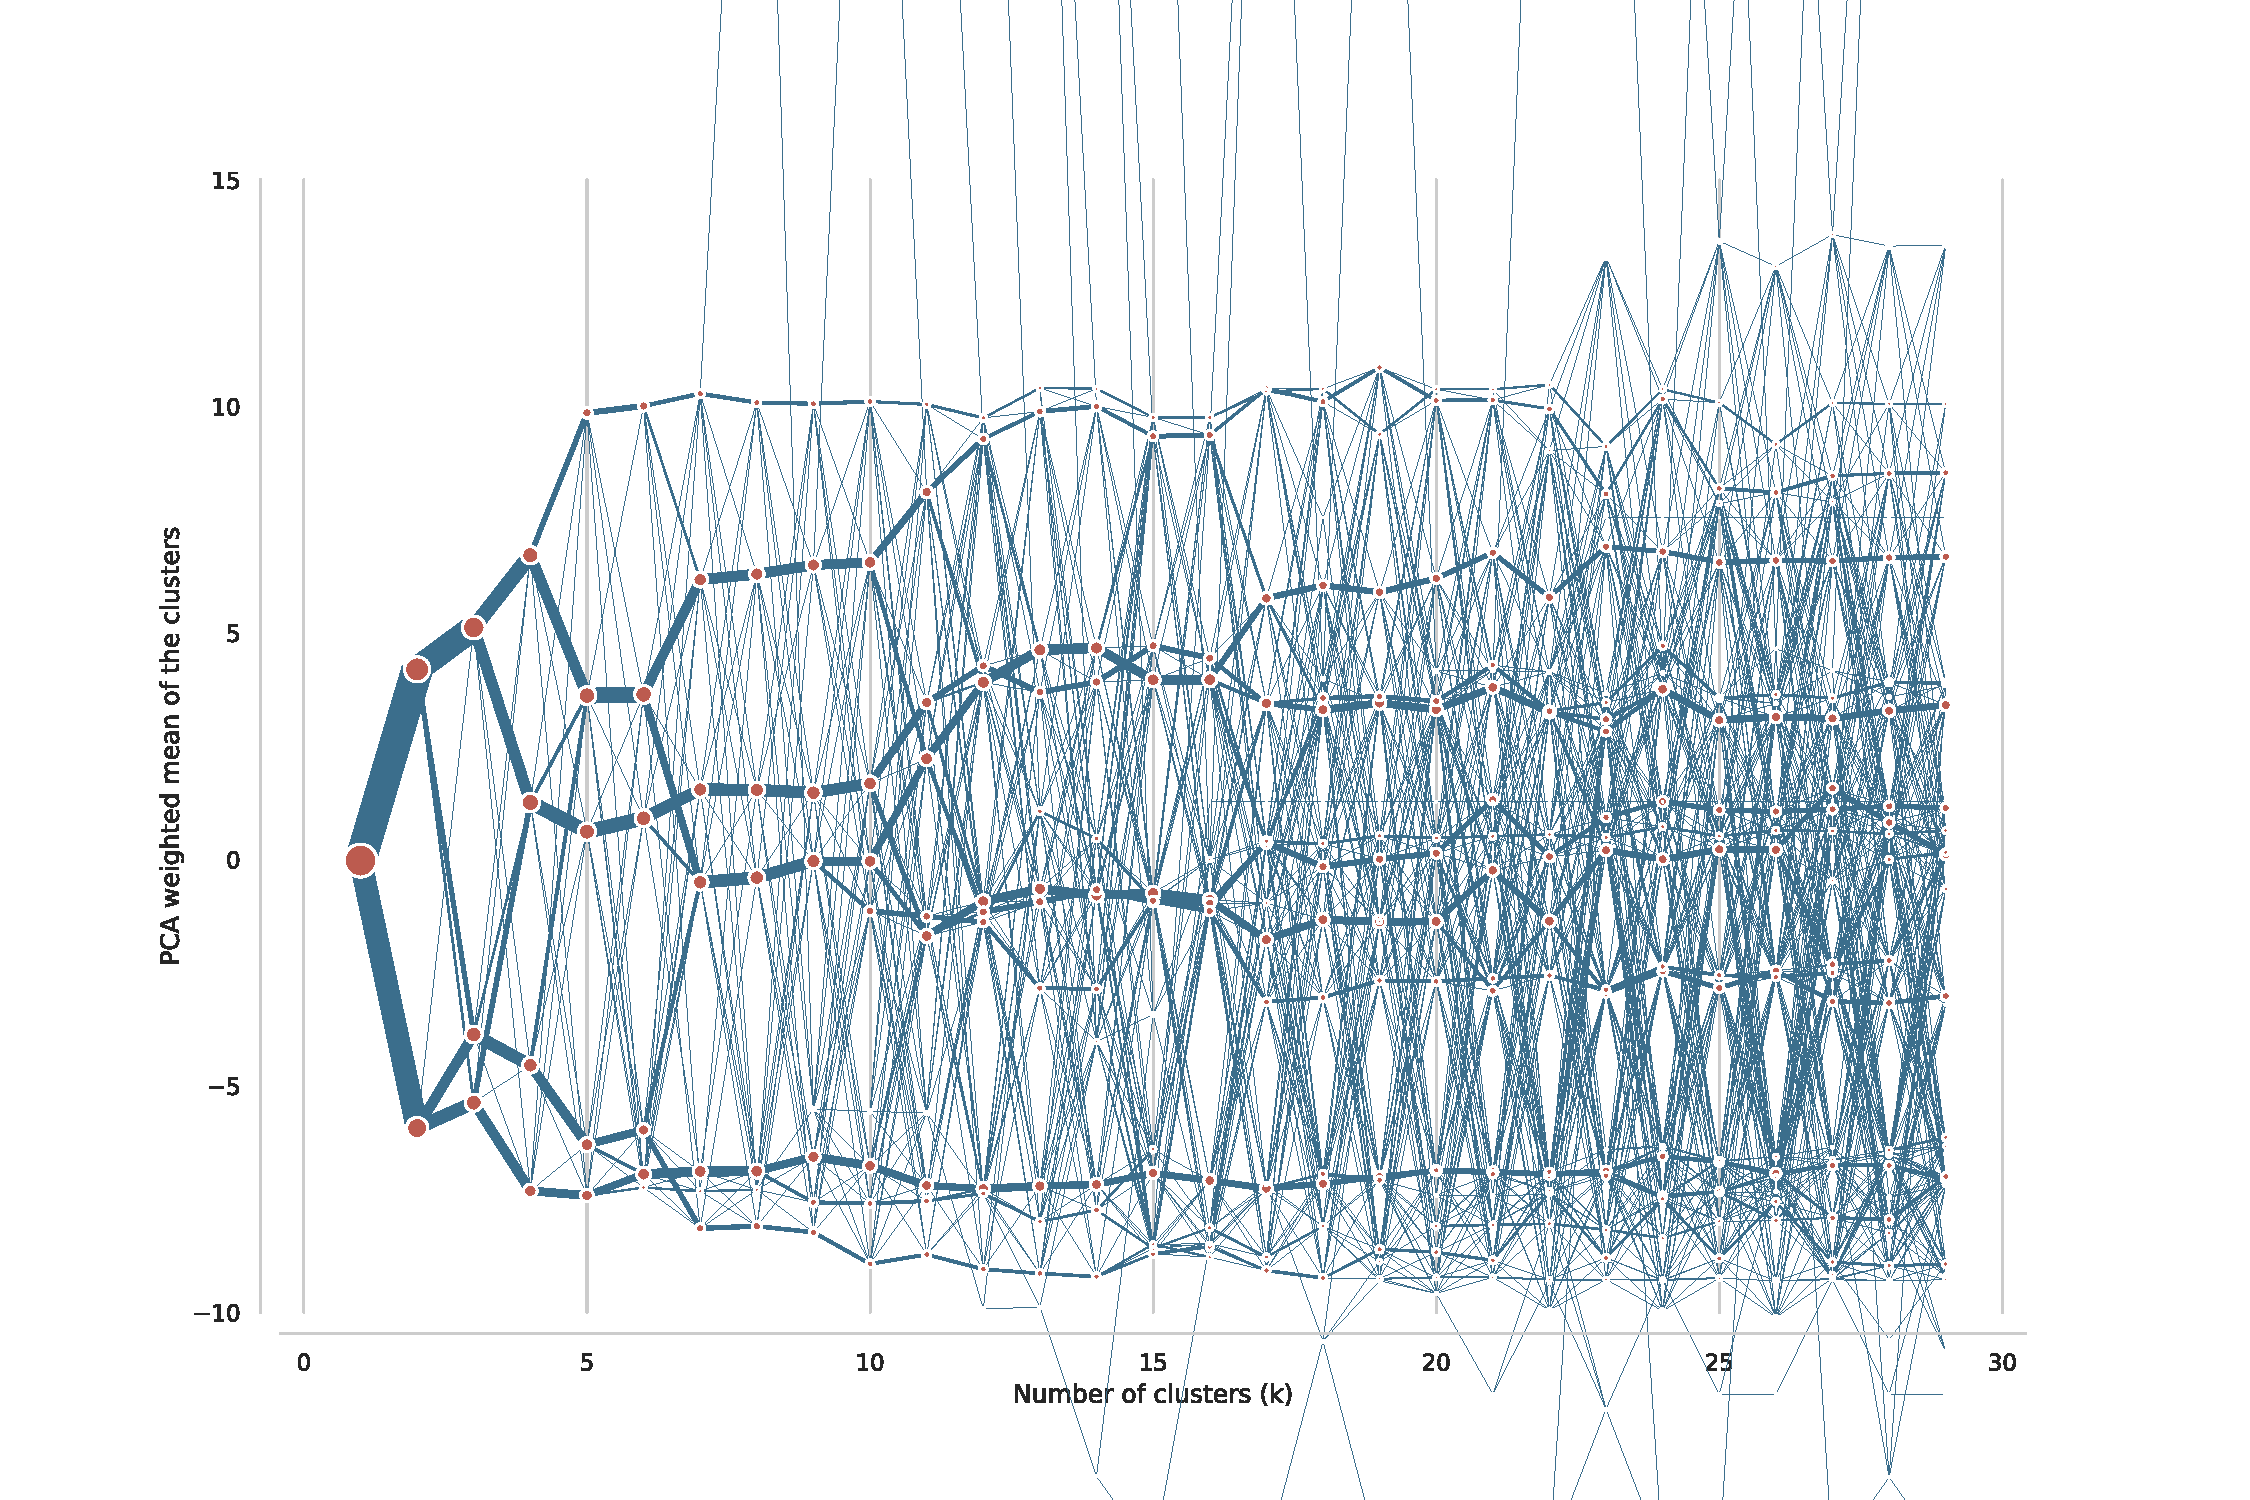
\includegraphics[width=\linewidth]{figures/clustergram_des.pdf}
    \caption{Clustergram (truncated along the vertical axis) illustrating the behaviour of dataset in different clustering options. The optimal number of clusters derived using the clustergram is 17.}
    \label{fig:cgram_des}
\end{figure}

\begin{figure}
    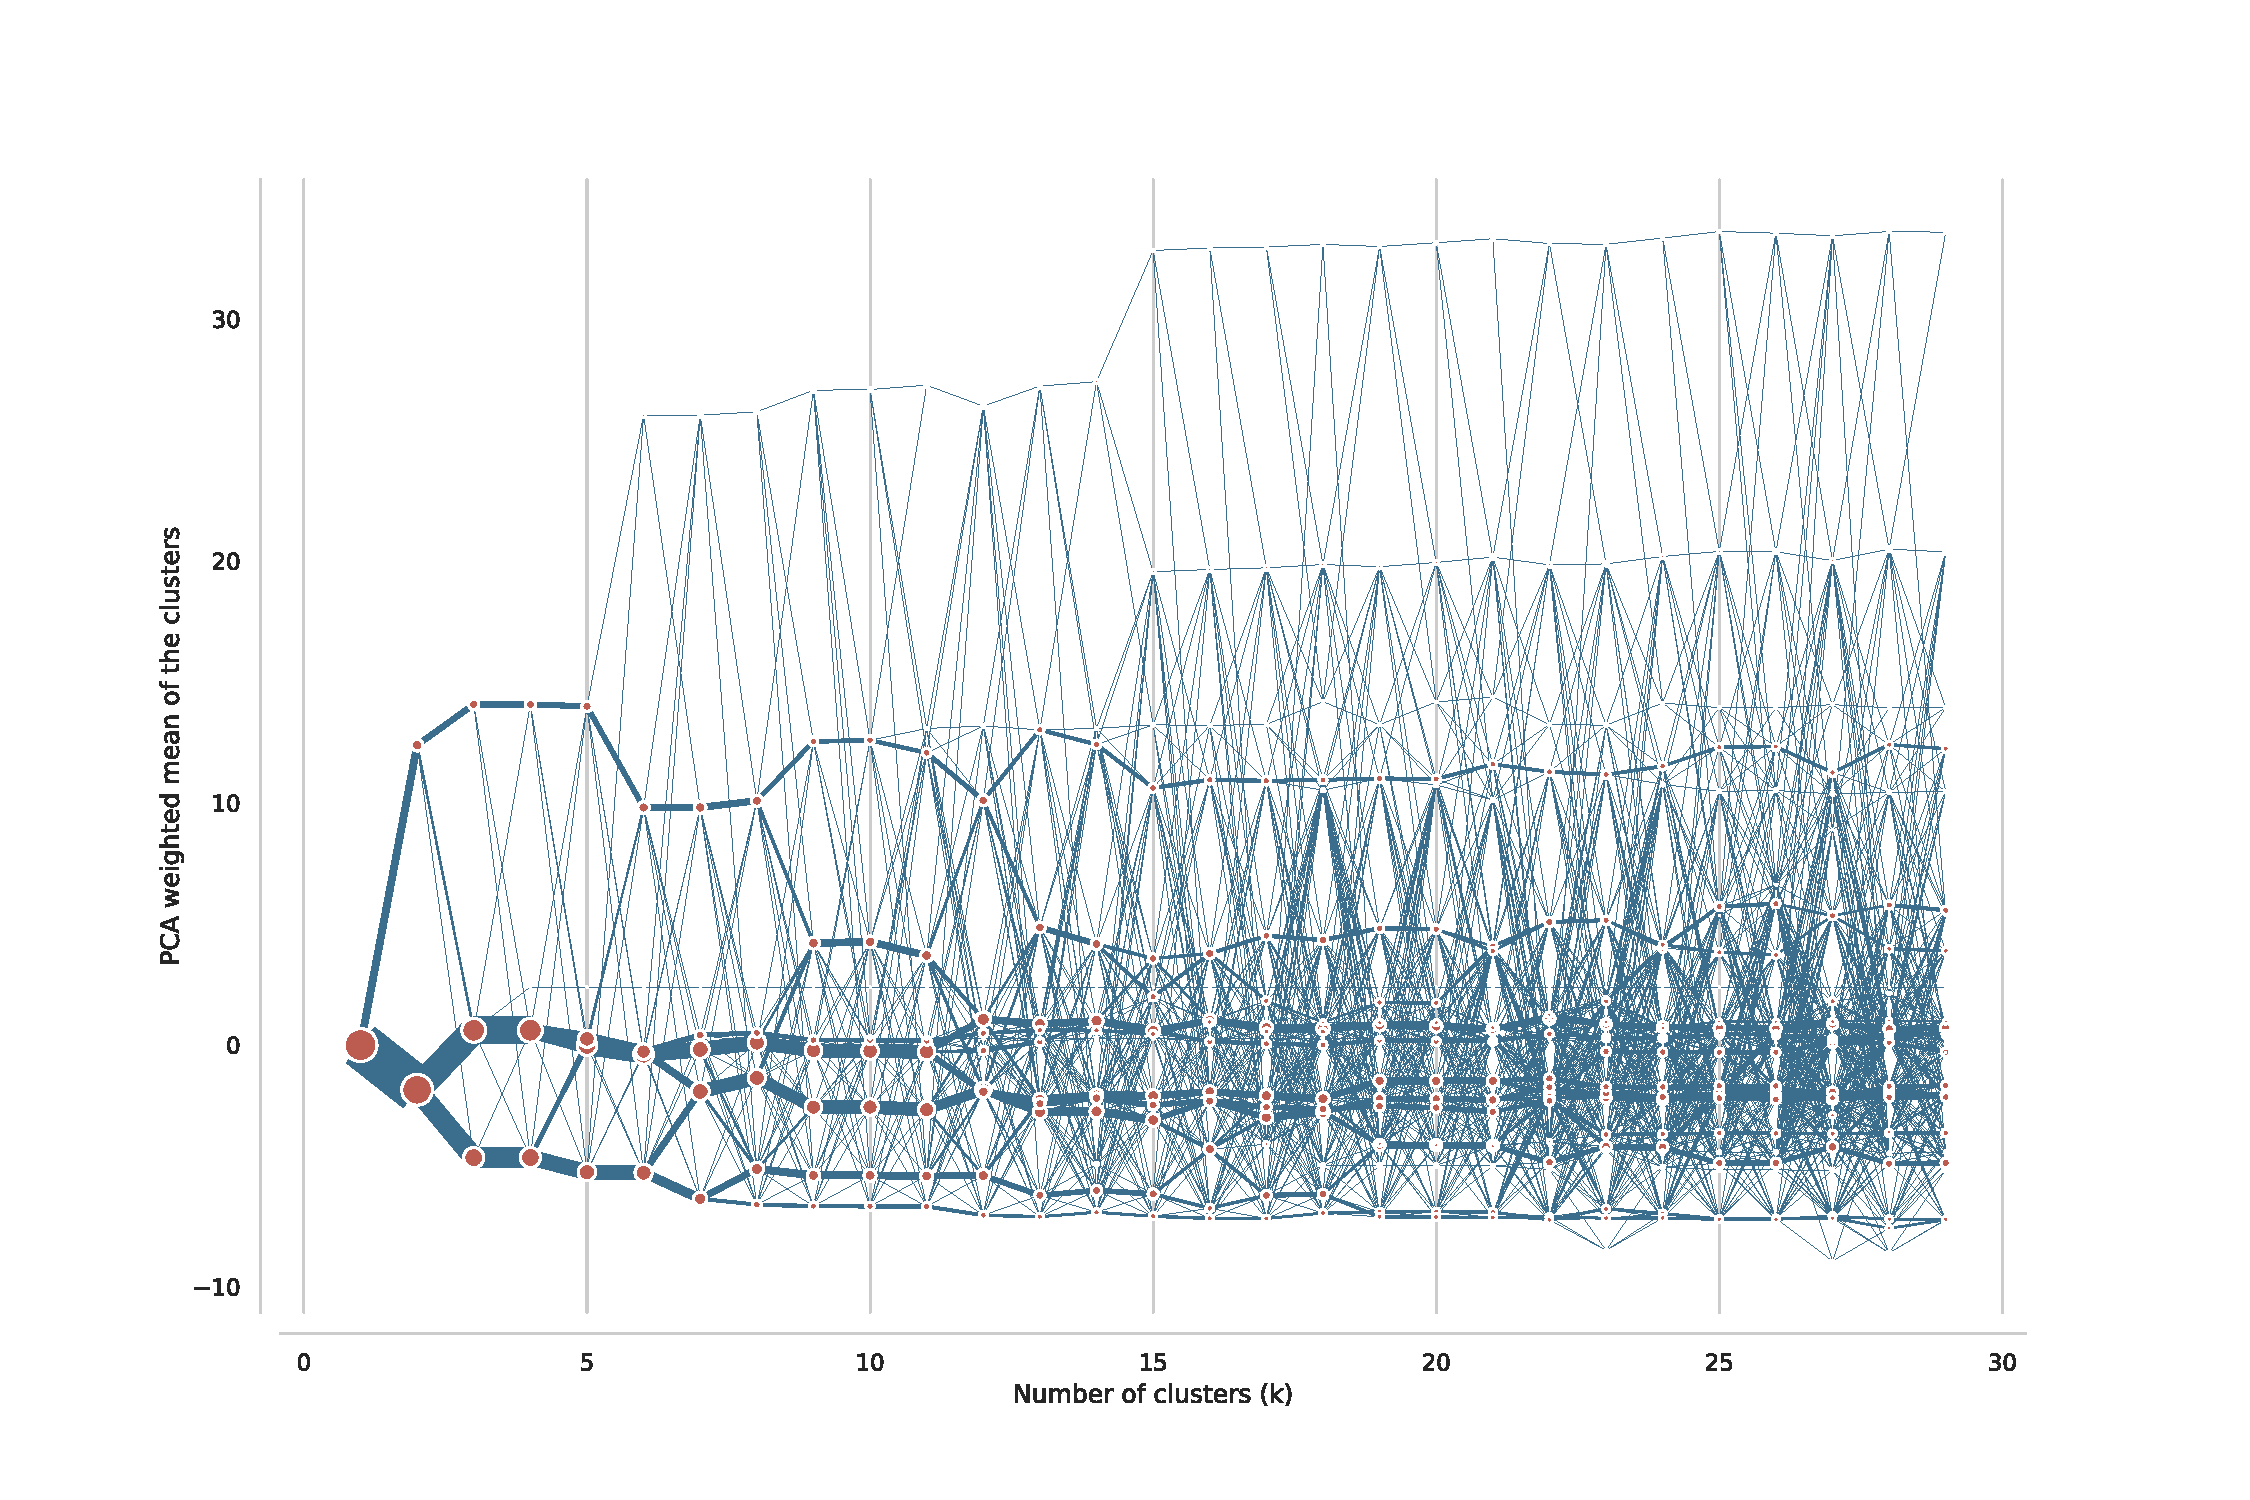
\includegraphics[width=\linewidth]{figures/clustergram_hou.pdf}
    \caption{Clustergram (truncated along the vertical axis) illustrating the behaviour of dataset in different clustering options. The optimal number of clusters derived using the clustergram is 9.}
    \label{fig:cgram_hou}
\end{figure}

\begin{figure}
    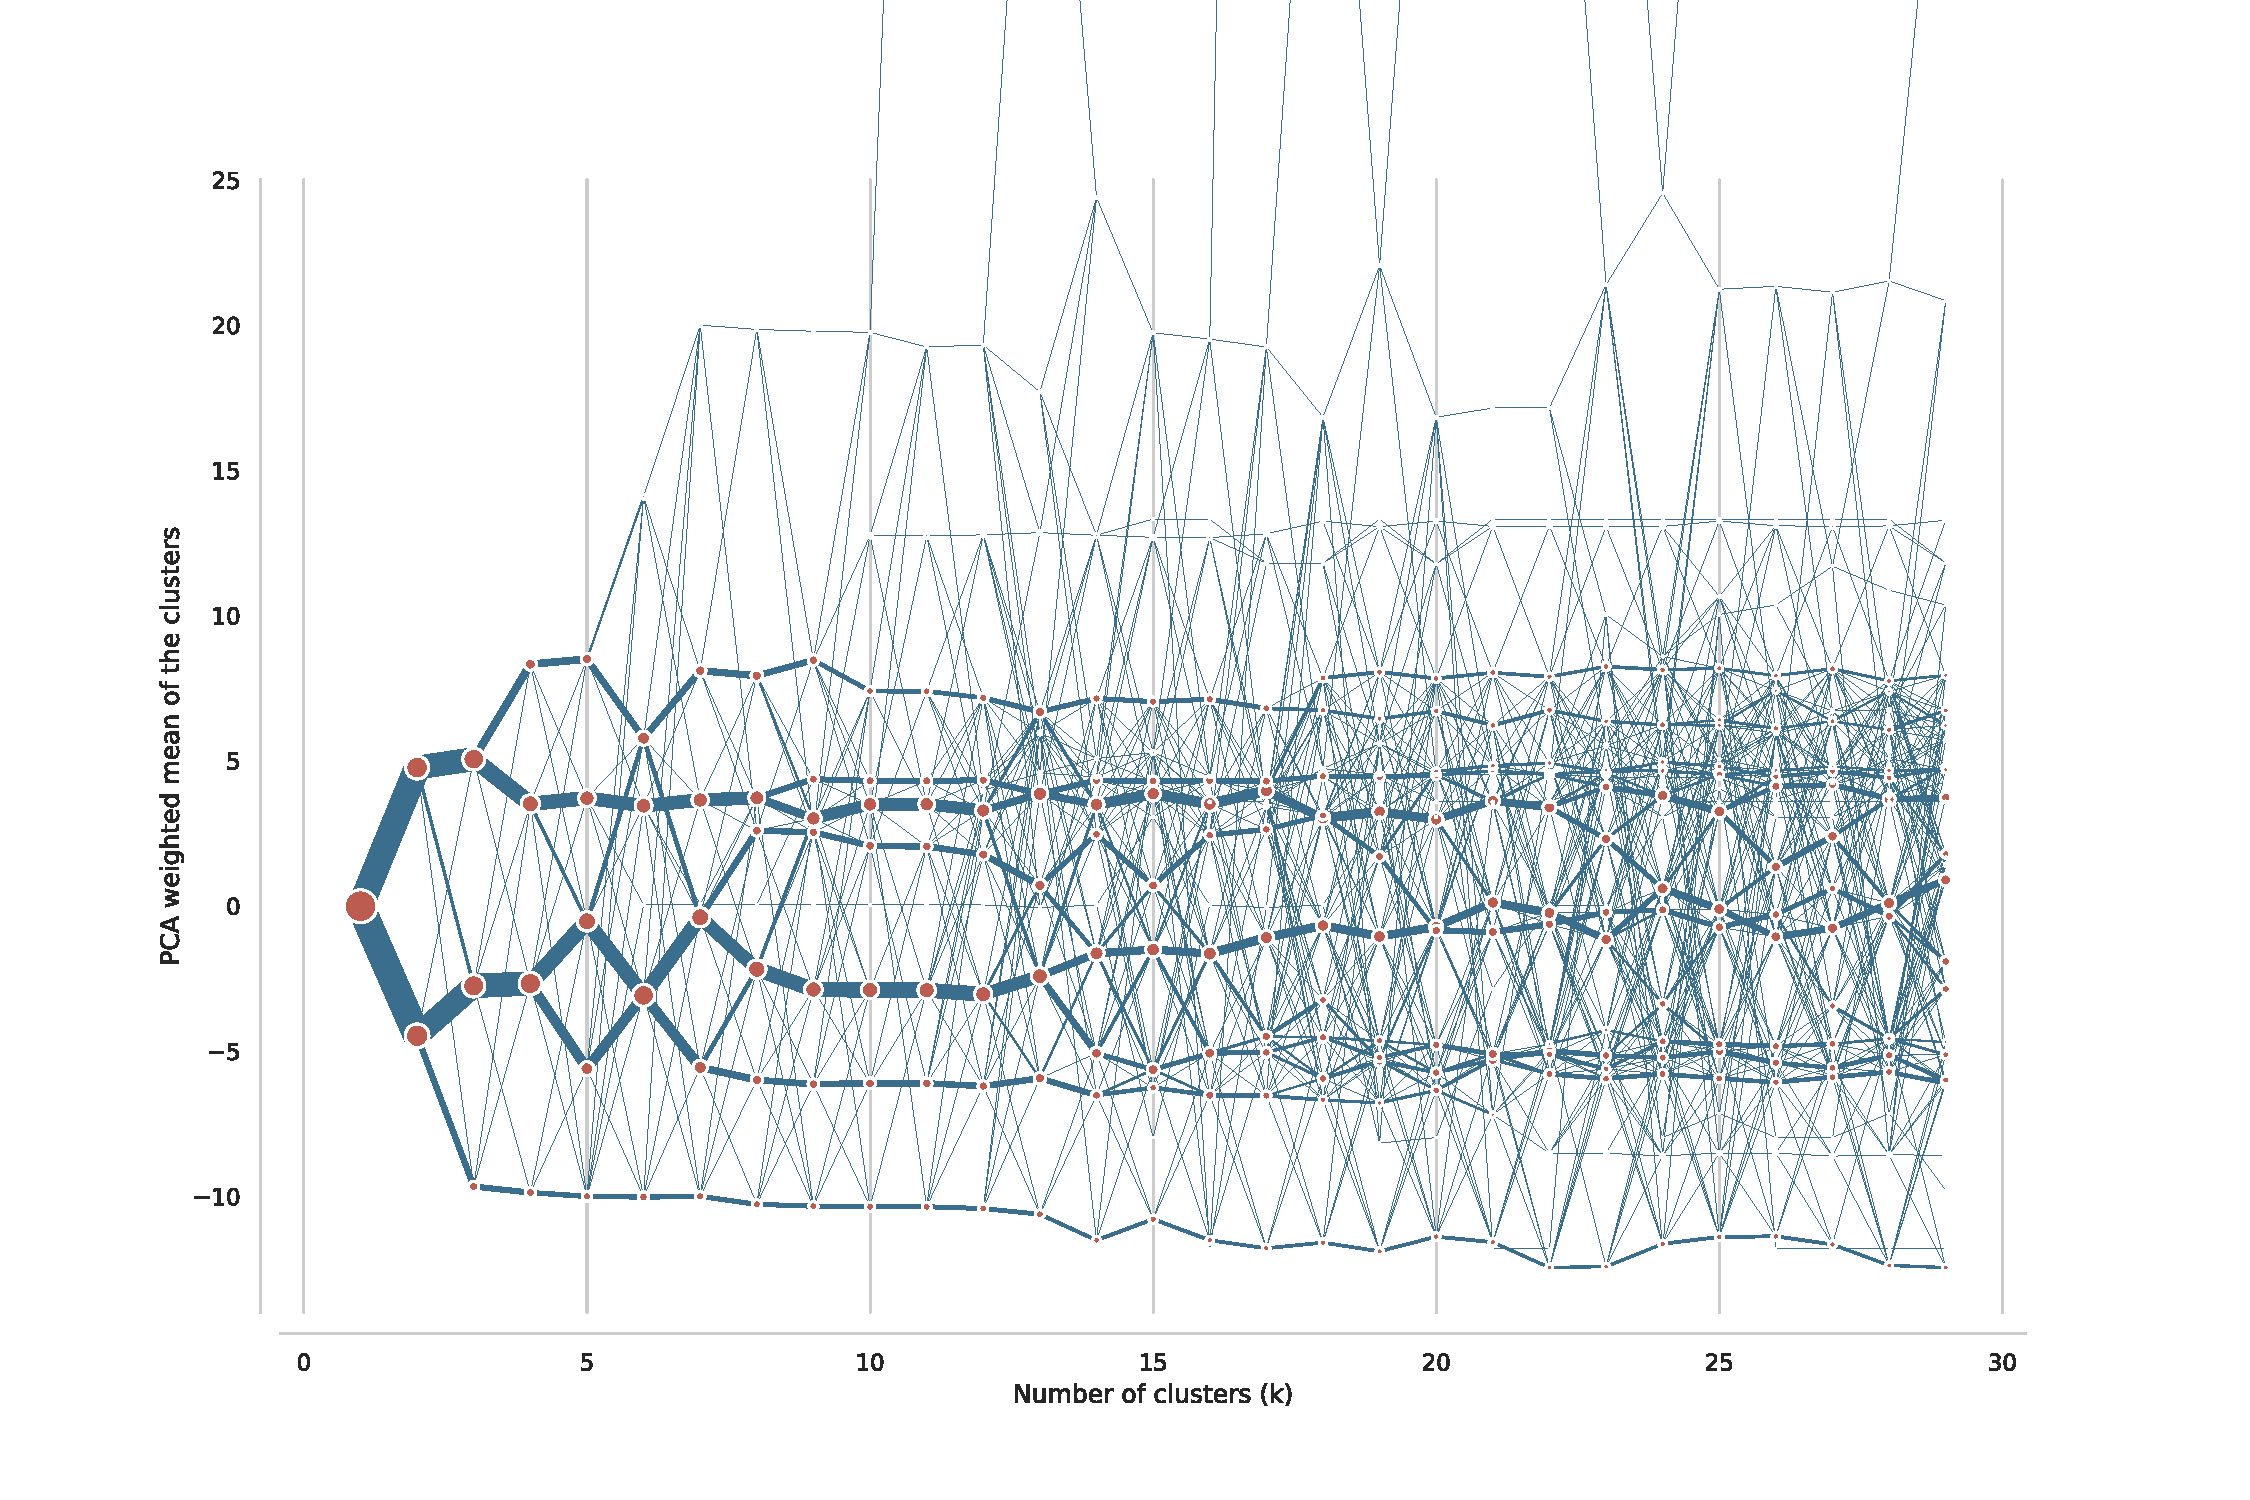
\includegraphics[width=\linewidth]{figures/clustergram_sin.pdf}
    \caption{Clustergram (truncated along the vertical axis) illustrating the behaviour of dataset in different clustering options. The optimal number of clusters derived using the clustergram is 16.}
    \label{fig:cgram_sin}
\end{figure}

\clearpage

\end{document}
